\documentclass[twoside]{book}

% Packages required by doxygen
\usepackage{fixltx2e}
\usepackage{calc}
\usepackage{doxygen}
\usepackage[export]{adjustbox} % also loads graphicx
\usepackage{graphicx}
\usepackage[utf8]{inputenc}
\usepackage{makeidx}
\usepackage{multicol}
\usepackage{multirow}
\PassOptionsToPackage{warn}{textcomp}
\usepackage{textcomp}
\usepackage[nointegrals]{wasysym}
\usepackage[table]{xcolor}

% Font selection
\usepackage[T1]{fontenc}
\usepackage[scaled=.90]{helvet}
\usepackage{courier}
\usepackage{amssymb}
\usepackage{sectsty}
\renewcommand{\familydefault}{\sfdefault}
\allsectionsfont{%
  \fontseries{bc}\selectfont%
  \color{darkgray}%
}
\renewcommand{\DoxyLabelFont}{%
  \fontseries{bc}\selectfont%
  \color{darkgray}%
}
\newcommand{\+}{\discretionary{\mbox{\scriptsize$\hookleftarrow$}}{}{}}

% Page & text layout
\usepackage{geometry}
\geometry{%
  a4paper,%
  top=2.5cm,%
  bottom=2.5cm,%
  left=2.5cm,%
  right=2.5cm%
}
\tolerance=750
\hfuzz=15pt
\hbadness=750
\setlength{\emergencystretch}{15pt}
\setlength{\parindent}{0cm}
\setlength{\parskip}{3ex plus 2ex minus 2ex}
\makeatletter
\renewcommand{\paragraph}{%
  \@startsection{paragraph}{4}{0ex}{-1.0ex}{1.0ex}{%
    \normalfont\normalsize\bfseries\SS@parafont%
  }%
}
\renewcommand{\subparagraph}{%
  \@startsection{subparagraph}{5}{0ex}{-1.0ex}{1.0ex}{%
    \normalfont\normalsize\bfseries\SS@subparafont%
  }%
}
\makeatother

% Headers & footers
\usepackage{fancyhdr}
\pagestyle{fancyplain}
\fancyhead[LE]{\fancyplain{}{\bfseries\thepage}}
\fancyhead[CE]{\fancyplain{}{}}
\fancyhead[RE]{\fancyplain{}{\bfseries\leftmark}}
\fancyhead[LO]{\fancyplain{}{\bfseries\rightmark}}
\fancyhead[CO]{\fancyplain{}{}}
\fancyhead[RO]{\fancyplain{}{\bfseries\thepage}}
\fancyfoot[LE]{\fancyplain{}{}}
\fancyfoot[CE]{\fancyplain{}{}}
\fancyfoot[RE]{\fancyplain{}{\bfseries\scriptsize Generated by Doxygen }}
\fancyfoot[LO]{\fancyplain{}{\bfseries\scriptsize Generated by Doxygen }}
\fancyfoot[CO]{\fancyplain{}{}}
\fancyfoot[RO]{\fancyplain{}{}}
\renewcommand{\footrulewidth}{0.4pt}
\renewcommand{\chaptermark}[1]{%
  \markboth{#1}{}%
}
\renewcommand{\sectionmark}[1]{%
  \markright{\thesection\ #1}%
}

% Indices & bibliography
\usepackage{natbib}
\usepackage[titles]{tocloft}
\setcounter{tocdepth}{3}
\setcounter{secnumdepth}{5}
\makeindex

% Hyperlinks (required, but should be loaded last)
\usepackage{ifpdf}
\ifpdf
  \usepackage[pdftex,pagebackref=true]{hyperref}
\else
  \usepackage[ps2pdf,pagebackref=true]{hyperref}
\fi
\hypersetup{%
  colorlinks=true,%
  linkcolor=blue,%
  citecolor=blue,%
  unicode%
}

% Custom commands
\newcommand{\clearemptydoublepage}{%
  \newpage{\pagestyle{empty}\cleardoublepage}%
}

\usepackage{caption}
\captionsetup{labelsep=space,justification=centering,font={bf},singlelinecheck=off,skip=4pt,position=top}

%===== C O N T E N T S =====

\begin{document}

% Titlepage & ToC
\hypersetup{pageanchor=false,
             bookmarksnumbered=true,
             pdfencoding=unicode
            }
\pagenumbering{alph}
\begin{titlepage}
\vspace*{7cm}
\begin{center}%
{\Large clibs }\\
\vspace*{1cm}
{\large Generated by Doxygen 1.8.13}\\
\end{center}
\end{titlepage}
\clearemptydoublepage
\pagenumbering{roman}
\tableofcontents
\clearemptydoublepage
\pagenumbering{arabic}
\hypersetup{pageanchor=true}

%--- Begin generated contents ---
\chapter{clibs}
\label{index}\hypertarget{index}{}\href{https://opensource.org/licenses/MIT}{\tt } \href{https://ci.appveyor.com/project/cwchentw/clibs}{\tt }

Tiny but handy utility libraries for C.

Visit the website of {\bfseries clibs} \href{https://cwchentw.github.io/clibs/html/index.html}{\tt here}.

Vist the repository of {\bfseries clibs} \href{https://github.com/cwchentw/clibs/}{\tt here}.

\subsection*{Warning}

D\+ON\textquotesingle{}T U\+SE IT IN P\+R\+O\+D\+U\+C\+T\+I\+ON E\+N\+V\+I\+R\+O\+N\+M\+E\+NT.

clibs is still experimental and for personal use only. The A\+PI may change without warning.

\subsection*{What is clibs anyway?}

{\bfseries clibs} are common utilities (types, macros, functions) used across C programs. They are mostly domain neutral, able to be applied to various situations.

\subsection*{System Requirements}


\begin{DoxyItemize}
\item A C compiler that supports A\+N\+SI C
\item ncurses (only for testing)
\end{DoxyItemize}

{\bfseries clibs} is written in A\+N\+SI C (C89). Nevertheless, We tested {\bfseries clibs} against C89, C99 and C11. Hence, you may use it for code in either A\+N\+SI C or modern C.

We tested {\bfseries clibs} against several Unix or Unix-\/like systems\+:


\begin{DoxyItemize}
\item Ubuntu 18.\+04 L\+TS
\item Cent\+OS 8
\item open\+S\+U\+SE Leap 15.\+1
\item True\+OS, Free\+B\+SD compatible
\item Solaris 11
\end{DoxyItemize}

It should work on other Unix or Unix-\/like systems as well.

B\+TW, though we didn\textquotesingle{}t test {\bfseries clibs} against Windows, it should also work because {\bfseries clibs} is implemented in A\+N\+SI C.

\subsection*{How to Use?}

The libraries in {\bfseries clibs} are self-\/contained, distributed in either single header or single header plus single source combo. Just copy what you need to your own C project.

test\+\_\+$\ast$.c are test programs. You don\textquotesingle{}t need them to use {\bfseries clibs}.

\subsection*{Available Utilities\+:}


\begin{DoxyItemize}
\item {\itshape \mbox{\hyperlink{boolean_8h}{boolean.\+h}}}\+: boolean type for C
\item {\itshape \mbox{\hyperlink{cmath_8h}{cmath.\+h}}}\+: basic math operations
\item {\itshape \mbox{\hyperlink{cstring_8h}{cstring.\+h}}} and {\itshape cstring.\+c}\+: utility functions for C strings (null-\/terminated {\ttfamily char} arrays)
\item {\itshape \mbox{\hyperlink{platform_8h}{platform.\+h}}}\+: platform-\/specific data
\item {\itshape \mbox{\hyperlink{print_8h}{print.\+h}}}\+: console printing related function-\/like macros
\item {\itshape \mbox{\hyperlink{term__color_8h}{term\+\_\+color.\+h}}}\+: console color related macros
\end{DoxyItemize}

Check the A\+PI of {\bfseries clibs} \href{https://cwchentw.github.io/clibs/html/index.html}{\tt here}.

\subsection*{Copyright}

Copyright (c) 2019 Michael Chen. Licensed under M\+IT. 
\chapter{T\+O\+DO}
\label{md_TODO}
\Hypertarget{md_TODO}

\begin{DoxyItemize}
\item Add {\ttfamily S\-Q\-U\-A\-R\-E(n)} macro
\item Refactor the project into a nested project
\item {\ttfamily cio} module for I/\-O as C string, i.\-e. null-\/terminated {\ttfamily char} array
\begin{DoxyItemize}
\item {\ttfamily stream\-\_\-read\-\_\-line} function to read stream line by line
\item {\ttfamily stream\-\_\-read\-\_\-all} function to read all text from stream
\item {\ttfamily cstring\-\_\-read\-\_\-line} function to read C string line by line
\end{DoxyItemize}
\item {\ttfamily path} module for file path cross Windows and Unix
\begin{DoxyItemize}
\item {\ttfamily base\-\_\-name} function to get base name of a file path
\item {\ttfamily dir\-\_\-name} function to get directory name of a file path
\item {\ttfamily ext\-\_\-name} function to get file extension of a file path 
\end{DoxyItemize}
\end{DoxyItemize}
\chapter{File Index}
\section{File List}
Here is a list of all documented files with brief descriptions\+:\begin{DoxyCompactList}
\item\contentsline{section}{\hyperlink{boolean_8h}{boolean.\+h} \\*Boolean type for C }{\pageref{boolean_8h}}{}
\item\contentsline{section}{\hyperlink{cmath_8h}{cmath.\+h} \\*Common math operations }{\pageref{cmath_8h}}{}
\item\contentsline{section}{\hyperlink{cstring_8h}{cstring.\+h} \\*Utility functions for C strings }{\pageref{cstring_8h}}{}
\item\contentsline{section}{\hyperlink{platform_8h}{platform.\+h} \\*Platform-\/specific data }{\pageref{platform_8h}}{}
\item\contentsline{section}{\hyperlink{print_8h}{print.\+h} \\*Console printing related macros }{\pageref{print_8h}}{}
\end{DoxyCompactList}

\chapter{File Documentation}
\hypertarget{boolean_8h}{}\section{boolean.\+h File Reference}
\label{boolean_8h}\index{boolean.\+h@{boolean.\+h}}


Boolean type for C.  


\subsection*{Macros}
\begin{DoxyCompactItemize}
\item 
\mbox{\Hypertarget{boolean_8h_aa93f0eb578d23995850d61f7d61c55c1}\label{boolean_8h_aa93f0eb578d23995850d61f7d61c55c1}} 
\#define \hyperlink{boolean_8h_aa93f0eb578d23995850d61f7d61c55c1}{F\+A\+L\+SE}~0
\begin{DoxyCompactList}\small\item\em False in boolean type. \end{DoxyCompactList}\item 
\mbox{\Hypertarget{boolean_8h_aa8cecfc5c5c054d2875c03e77b7be15d}\label{boolean_8h_aa8cecfc5c5c054d2875c03e77b7be15d}} 
\#define \hyperlink{boolean_8h_aa8cecfc5c5c054d2875c03e77b7be15d}{T\+R\+UE}~1
\begin{DoxyCompactList}\small\item\em True in boolean type. \end{DoxyCompactList}\item 
\mbox{\Hypertarget{boolean_8h_af7c650f18c4f6a93c33638cf9426b216}\label{boolean_8h_af7c650f18c4f6a93c33638cf9426b216}} 
\#define {\bfseries \+\_\+\+B\+O\+O\+L\+\_\+\+I\+S\+\_\+\+D\+E\+F\+I\+N\+ED}
\end{DoxyCompactItemize}
\subsection*{Typedefs}
\begin{DoxyCompactItemize}
\item 
\mbox{\Hypertarget{boolean_8h_a3e5b8192e7d9ffaf3542f1210aec18dd}\label{boolean_8h_a3e5b8192e7d9ffaf3542f1210aec18dd}} 
typedef unsigned char \hyperlink{boolean_8h_a3e5b8192e7d9ffaf3542f1210aec18dd}{B\+O\+OL}
\begin{DoxyCompactList}\small\item\em Custom boolean type. \end{DoxyCompactList}\end{DoxyCompactItemize}


\subsection{Detailed Description}
Boolean type for C. 

\begin{DoxyAuthor}{Author}
OpenTechCoder 
\end{DoxyAuthor}
\begin{DoxyCopyright}{Copyright}
M\+IT
\end{DoxyCopyright}
Win32 A\+PI provides its own {\bfseries B\+O\+OL} type. Hence, this header is useless in Win32 A\+PI programming. 
\hypertarget{cio_8h}{}\doxysection{cio.\+h File Reference}
\label{cio_8h}\index{cio.h@{cio.h}}


Basic input and output for C.  


{\ttfamily \#include $<$stdio.\+h$>$}\newline
Include dependency graph for cio.\+h\+:\nopagebreak
\begin{figure}[H]
\begin{center}
\leavevmode
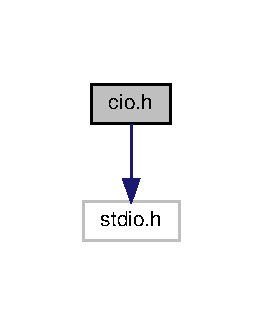
\includegraphics[width=125pt]{cio_8h__incl}
\end{center}
\end{figure}
\doxysubsection*{Functions}
\begin{DoxyCompactItemize}
\item 
char $\ast$ \mbox{\hyperlink{cio_8h_a3976a75b6c155bc57f41586f0a3bd503}{stream\+\_\+read\+\_\+all}} (F\+I\+LE $\ast$fp)
\begin{DoxyCompactList}\small\item\em Read all the content of {\itshape fp} into C string. \end{DoxyCompactList}\end{DoxyCompactItemize}


\doxysubsection{Detailed Description}
Basic input and output for C. 

\begin{DoxyAuthor}{Author}
Michael Chen 
\end{DoxyAuthor}
\begin{DoxyCopyright}{Copyright}
M\+IT 
\end{DoxyCopyright}


\doxysubsection{Function Documentation}
\mbox{\Hypertarget{cio_8h_a3976a75b6c155bc57f41586f0a3bd503}\label{cio_8h_a3976a75b6c155bc57f41586f0a3bd503}} 
\index{cio.h@{cio.h}!stream\_read\_all@{stream\_read\_all}}
\index{stream\_read\_all@{stream\_read\_all}!cio.h@{cio.h}}
\doxysubsubsection{\texorpdfstring{stream\_read\_all()}{stream\_read\_all()}}
{\footnotesize\ttfamily char$\ast$ stream\+\_\+read\+\_\+all (\begin{DoxyParamCaption}\item[{F\+I\+LE $\ast$}]{fp }\end{DoxyParamCaption})}



Read all the content of {\itshape fp} into C string. 


\begin{DoxyParams}{Parameters}
{\em fp} & a i/o stream \\
\hline
\end{DoxyParams}
\begin{DoxyReturn}{Returns}
char $\ast$ 
\end{DoxyReturn}

\hypertarget{clibs__math_8h}{}\doxysection{clibs\+\_\+math.\+h File Reference}
\label{clibs__math_8h}\index{clibs\_math.h@{clibs\_math.h}}


Common math operations.  


\doxysubsection*{Macros}
\begin{DoxyCompactItemize}
\item 
\mbox{\Hypertarget{clibs__math_8h_afa99ec4acc4ecb2dc3c2d05da15d0e3f}\label{clibs__math_8h_afa99ec4acc4ecb2dc3c2d05da15d0e3f}} 
\#define \mbox{\hyperlink{clibs__math_8h_afa99ec4acc4ecb2dc3c2d05da15d0e3f}{M\+AX}}(a,  b)~((a) $>$ (b) ? (a) \+: (b))
\begin{DoxyCompactList}\small\item\em Get the maximal value between {\itshape a} and {\itshape b}. \end{DoxyCompactList}\item 
\mbox{\Hypertarget{clibs__math_8h_a3acffbd305ee72dcd4593c0d8af64a4f}\label{clibs__math_8h_a3acffbd305ee72dcd4593c0d8af64a4f}} 
\#define \mbox{\hyperlink{clibs__math_8h_a3acffbd305ee72dcd4593c0d8af64a4f}{M\+IN}}(a,  b)~((a) $<$ (b) ? (a) \+: (b))
\begin{DoxyCompactList}\small\item\em Get the minimal value between {\itshape a} and {\itshape b}. \end{DoxyCompactList}\item 
\mbox{\Hypertarget{clibs__math_8h_ae2f08dc603ae93c402abd918ba4e23e1}\label{clibs__math_8h_ae2f08dc603ae93c402abd918ba4e23e1}} 
\#define \mbox{\hyperlink{clibs__math_8h_ae2f08dc603ae93c402abd918ba4e23e1}{A\+BS}}(a)~((a) $>$ 0.\+0 ? (a) \+: -\/(a))
\begin{DoxyCompactList}\small\item\em Get the absolute value of {\itshape a}. \end{DoxyCompactList}\item 
\#define \mbox{\hyperlink{clibs__math_8h_a8eb7da27bde11ccd5bf0c204ad32fb89}{E\+Q\+U\+AL}}(a,  b)
\begin{DoxyCompactList}\small\item\em Check the equality between two floating-\/point numbers. \end{DoxyCompactList}\item 
\mbox{\Hypertarget{clibs__math_8h_aff5407859c02b1b107d77a0b26ccfa20}\label{clibs__math_8h_aff5407859c02b1b107d77a0b26ccfa20}} 
\#define \mbox{\hyperlink{clibs__math_8h_aff5407859c02b1b107d77a0b26ccfa20}{I\+S\+\_\+\+E\+V\+EN}}(n)~(0 == ((n) \& 1))
\begin{DoxyCompactList}\small\item\em Check whether {\itshape n} is even. \end{DoxyCompactList}\item 
\mbox{\Hypertarget{clibs__math_8h_a0fac5864e00584bf98923b4c2dc497f9}\label{clibs__math_8h_a0fac5864e00584bf98923b4c2dc497f9}} 
\#define \mbox{\hyperlink{clibs__math_8h_a0fac5864e00584bf98923b4c2dc497f9}{I\+S\+\_\+\+O\+DD}}(n)~(1 == ((n) \& 1))
\begin{DoxyCompactList}\small\item\em Check whether {\itshape n} is odd. \end{DoxyCompactList}\item 
\#define \mbox{\hyperlink{clibs__math_8h_aac9153aee4bdb92701df902e06a74eb3}{S\+W\+AP}}(a,  b)~(((a) $^\wedge$= (b)), ((b) $^\wedge$= (a)), ((a) $^\wedge$= (b)))
\begin{DoxyCompactList}\small\item\em Swap between {\itshape a} and {\itshape b}. \end{DoxyCompactList}\end{DoxyCompactItemize}


\doxysubsection{Detailed Description}
Common math operations. 

\begin{DoxyAuthor}{Author}
Michael Chen 
\end{DoxyAuthor}
\begin{DoxyCopyright}{Copyright}
M\+IT 
\end{DoxyCopyright}


\doxysubsection{Macro Definition Documentation}
\mbox{\Hypertarget{clibs__math_8h_a8eb7da27bde11ccd5bf0c204ad32fb89}\label{clibs__math_8h_a8eb7da27bde11ccd5bf0c204ad32fb89}} 
\index{clibs\_math.h@{clibs\_math.h}!EQUAL@{EQUAL}}
\index{EQUAL@{EQUAL}!clibs\_math.h@{clibs\_math.h}}
\doxysubsubsection{\texorpdfstring{EQUAL}{EQUAL}}
{\footnotesize\ttfamily \#define E\+Q\+U\+AL(\begin{DoxyParamCaption}\item[{}]{a,  }\item[{}]{b }\end{DoxyParamCaption})}

{\bfseries Value\+:}
\begin{DoxyCode}{0}
\DoxyCodeLine{(\textcolor{keyword}{sizeof}((a)) == 16 ? \mbox{\hyperlink{clibs__math_8h_ae2f08dc603ae93c402abd918ba4e23e1}{ABS}}((a) -\/ (b)) <= 0.000000000000000000000001 : \(\backslash\)}
\DoxyCodeLine{         (\textcolor{keyword}{sizeof}((a)) == 8 ? \mbox{\hyperlink{clibs__math_8h_ae2f08dc603ae93c402abd918ba4e23e1}{ABS}}((a) -\/ (b)) <= 0.000000000000001 : \(\backslash\)}
\DoxyCodeLine{                             ABS((a) -\/ (b)) <= 0.0000001))}

\end{DoxyCode}


Check the equality between two floating-\/point numbers. 

{\bfseries{\mbox{\hyperlink{clibs__math_8h_a8eb7da27bde11ccd5bf0c204ad32fb89}{E\+Q\+U\+A\+L(a, b)}}}} compares two floating-\/point numbers by the absolute value of the difference between them. The value should be small enough to be viewed as equal. {\bfseries{\mbox{\hyperlink{clibs__math_8h_a8eb7da27bde11ccd5bf0c204ad32fb89}{E\+Q\+U\+A\+L(a, b)}}}} utilizes {\bfseries{sizeof}} to get the width of the number to be compared so that it can compute a proper error value.


\begin{DoxyItemize}
\item float\+: 24 bit -\/$>$ 7 digits
\item double\+: 53 bit -\/$>$ 15 digits
\item long double\+: 80 bit -\/$>$ 24 digits
\end{DoxyItemize}

Formula to get the precision of each data type\+: \begin{DoxyVerb}digit = bit * log(2) / log(10)
\end{DoxyVerb}
 \mbox{\Hypertarget{clibs__math_8h_aac9153aee4bdb92701df902e06a74eb3}\label{clibs__math_8h_aac9153aee4bdb92701df902e06a74eb3}} 
\index{clibs\_math.h@{clibs\_math.h}!SWAP@{SWAP}}
\index{SWAP@{SWAP}!clibs\_math.h@{clibs\_math.h}}
\doxysubsubsection{\texorpdfstring{SWAP}{SWAP}}
{\footnotesize\ttfamily \#define S\+W\+AP(\begin{DoxyParamCaption}\item[{}]{a,  }\item[{}]{b }\end{DoxyParamCaption})~(((a) $^\wedge$= (b)), ((b) $^\wedge$= (a)), ((a) $^\wedge$= (b)))}



Swap between {\itshape a} and {\itshape b}. 

{\itshape a} and {\itshape b} are integers 
\hypertarget{clibs__time_8h}{}\section{clibs\+\_\+time.\+h File Reference}
\label{clibs__time_8h}\index{clibs\+\_\+time.\+h@{clibs\+\_\+time.\+h}}


Common time operations.  


{\ttfamily \#include $<$time.\+h$>$}\newline
Include dependency graph for clibs\+\_\+time.\+h\+:
\nopagebreak
\begin{figure}[H]
\begin{center}
\leavevmode
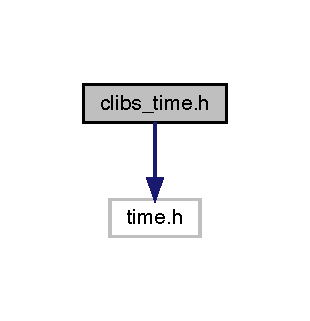
\includegraphics[width=149pt]{clibs__time_8h__incl}
\end{center}
\end{figure}
\subsection*{Functions}
\begin{DoxyCompactItemize}
\item 
struct tm \hyperlink{clibs__time_8h_aad8adbc23ac66ccf954bcd462bf1fa03}{date\+\_\+create} (int year, int month, int day)
\begin{DoxyCompactList}\small\item\em Create a date object. \end{DoxyCompactList}\item 
struct tm \hyperlink{clibs__time_8h_a7a8ff1bc3274e8a77fb73b5800d211e7}{time\+\_\+create} (int year, int month, int day, int hour, int min, int sec)
\begin{DoxyCompactList}\small\item\em Create a time object. \end{DoxyCompactList}\end{DoxyCompactItemize}


\subsection{Detailed Description}
Common time operations. 

\begin{DoxyAuthor}{Author}
Michael Chen 
\end{DoxyAuthor}
\begin{DoxyCopyright}{Copyright}
M\+IT 
\end{DoxyCopyright}


\subsection{Function Documentation}
\mbox{\Hypertarget{clibs__time_8h_aad8adbc23ac66ccf954bcd462bf1fa03}\label{clibs__time_8h_aad8adbc23ac66ccf954bcd462bf1fa03}} 
\index{clibs\+\_\+time.\+h@{clibs\+\_\+time.\+h}!date\+\_\+create@{date\+\_\+create}}
\index{date\+\_\+create@{date\+\_\+create}!clibs\+\_\+time.\+h@{clibs\+\_\+time.\+h}}
\subsubsection{\texorpdfstring{date\+\_\+create()}{date\_create()}}
{\footnotesize\ttfamily struct tm date\+\_\+create (\begin{DoxyParamCaption}\item[{int}]{year,  }\item[{int}]{month,  }\item[{int}]{day }\end{DoxyParamCaption})}



Create a date object. 


\begin{DoxyParams}{Parameters}
{\em year} & year in Gregorian calendar \\
\hline
{\em month} & from 1 to 12 \\
\hline
{\em day} & from 1 to 31 \\
\hline
\end{DoxyParams}
\begin{DoxyReturn}{Returns}
struct tm
\end{DoxyReturn}
Time is kept at 9\+:00 AM. \mbox{\Hypertarget{clibs__time_8h_a7a8ff1bc3274e8a77fb73b5800d211e7}\label{clibs__time_8h_a7a8ff1bc3274e8a77fb73b5800d211e7}} 
\index{clibs\+\_\+time.\+h@{clibs\+\_\+time.\+h}!time\+\_\+create@{time\+\_\+create}}
\index{time\+\_\+create@{time\+\_\+create}!clibs\+\_\+time.\+h@{clibs\+\_\+time.\+h}}
\subsubsection{\texorpdfstring{time\+\_\+create()}{time\_create()}}
{\footnotesize\ttfamily struct tm time\+\_\+create (\begin{DoxyParamCaption}\item[{int}]{year,  }\item[{int}]{month,  }\item[{int}]{day,  }\item[{int}]{hour,  }\item[{int}]{min,  }\item[{int}]{sec }\end{DoxyParamCaption})}



Create a time object. 


\begin{DoxyParams}{Parameters}
{\em year} & year in Gregorian calendar \\
\hline
{\em month} & from 1 to 12 \\
\hline
{\em day} & from 1 to 31 \\
\hline
{\em hour} & from 0 to 23 \\
\hline
{\em min} & from 0 to 59 \\
\hline
{\em sec} & from 0 to 59 \\
\hline
\end{DoxyParams}
\begin{DoxyReturn}{Returns}
struct tm 
\end{DoxyReturn}

\hypertarget{cstring_8h}{}\section{cstring.\+h File Reference}
\label{cstring_8h}\index{cstring.\+h@{cstring.\+h}}


Utility functions for C strings.  


{\ttfamily \#include $<$stdio.\+h$>$}\newline
Include dependency graph for cstring.\+h\+:\nopagebreak
\begin{figure}[H]
\begin{center}
\leavevmode
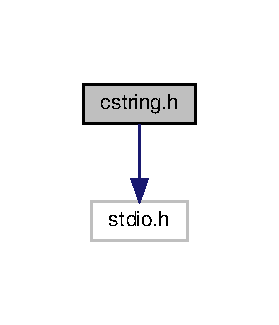
\includegraphics[width=134pt]{cstring_8h__incl}
\end{center}
\end{figure}
\subsection*{Macros}
\begin{DoxyCompactItemize}
\item 
\mbox{\Hypertarget{cstring_8h_aa93f0eb578d23995850d61f7d61c55c1}\label{cstring_8h_aa93f0eb578d23995850d61f7d61c55c1}} 
\#define {\bfseries F\+A\+L\+SE}~0
\item 
\mbox{\Hypertarget{cstring_8h_aa8cecfc5c5c054d2875c03e77b7be15d}\label{cstring_8h_aa8cecfc5c5c054d2875c03e77b7be15d}} 
\#define {\bfseries T\+R\+UE}~1
\item 
\mbox{\Hypertarget{cstring_8h_a1ca888bd091694c05472e1b91df1a97b}\label{cstring_8h_a1ca888bd091694c05472e1b91df1a97b}} 
\#define {\bfseries D\+L\+L\+\_\+\+E\+X\+P\+O\+RT}
\end{DoxyCompactItemize}
\subsection*{Typedefs}
\begin{DoxyCompactItemize}
\item 
\mbox{\Hypertarget{cstring_8h_af492d2bddcb2befacb3aa03dcdf9aafd}\label{cstring_8h_af492d2bddcb2befacb3aa03dcdf9aafd}} 
typedef char {\bfseries B\+O\+OL}
\end{DoxyCompactItemize}
\subsection*{Functions}
\begin{DoxyCompactItemize}
\item 
D\+L\+L\+\_\+\+E\+X\+P\+O\+RT \hyperlink{boolean_8h_a3e5b8192e7d9ffaf3542f1210aec18dd}{B\+O\+OL} \hyperlink{cstring_8h_a788b79461659ad8e79a9164af28d8ef2}{string\+\_\+is\+\_\+equal} (const char $\ast$a, const char $\ast$b)
\begin{DoxyCompactList}\small\item\em Check whether two strings are equal. \end{DoxyCompactList}\item 
D\+L\+L\+\_\+\+E\+X\+P\+O\+RT \hyperlink{boolean_8h_a3e5b8192e7d9ffaf3542f1210aec18dd}{B\+O\+OL} \hyperlink{cstring_8h_ad17149d107c4366f280da504df45cc10}{string\+\_\+starts\+\_\+with} (const char $\ast$a, const char $\ast$b)
\begin{DoxyCompactList}\small\item\em Check whether string {\itshape a} starts with string {\itshape b}. \end{DoxyCompactList}\item 
D\+L\+L\+\_\+\+E\+X\+P\+O\+RT \hyperlink{boolean_8h_a3e5b8192e7d9ffaf3542f1210aec18dd}{B\+O\+OL} \hyperlink{cstring_8h_ae0bb75ef00bf73fe720b76c56c98325f}{string\+\_\+contains} (const char $\ast$a, const char $\ast$b)
\begin{DoxyCompactList}\small\item\em Check whether string {\itshape a} contains string {\itshape b}. \end{DoxyCompactList}\item 
D\+L\+L\+\_\+\+E\+X\+P\+O\+RT \hyperlink{boolean_8h_a3e5b8192e7d9ffaf3542f1210aec18dd}{B\+O\+OL} \hyperlink{cstring_8h_a4b78c493fbd5c995fd8b1edc5067caf2}{string\+\_\+is\+\_\+space\+\_\+only} (const char $\ast$s)
\begin{DoxyCompactList}\small\item\em Check whether string {\itshape s} composes of only spaces. \end{DoxyCompactList}\item 
D\+L\+L\+\_\+\+E\+X\+P\+O\+RT char $\ast$ \hyperlink{cstring_8h_a5594f2b0ce2c840820c0a28fc44b7956}{string\+\_\+allocate} (const char $\ast$s)
\begin{DoxyCompactList}\small\item\em Allocate a new string out of string {\itshape s}. \end{DoxyCompactList}\item 
D\+L\+L\+\_\+\+E\+X\+P\+O\+RT char $\ast$ \hyperlink{cstring_8h_a4f33944441c46a997af3ebd1eeed1e82}{string\+\_\+allocate\+\_\+substring} (const char $\ast$s, size\+\_\+t from, size\+\_\+t to)
\begin{DoxyCompactList}\small\item\em Allocate a new substring out of string {\itshape s} from {\itshape from} to {\itshape to}. \end{DoxyCompactList}\item 
D\+L\+L\+\_\+\+E\+X\+P\+O\+RT F\+I\+LE $\ast$ \hyperlink{cstring_8h_a28b2afbc73cc0806bbec57eb1da1d6ec}{string\+\_\+to\+\_\+stream} (char $\ast$s)
\begin{DoxyCompactList}\small\item\em Convert a string to a file stream. \end{DoxyCompactList}\end{DoxyCompactItemize}


\subsection{Detailed Description}
Utility functions for C strings. 

\begin{DoxyAuthor}{Author}
Michael Chen 
\end{DoxyAuthor}
\begin{DoxyCopyright}{Copyright}
M\+IT
\end{DoxyCopyright}
{\bfseries \hyperlink{cstring_8h}{cstring.\+h}} and {\bfseries cstring.\+c} only support null-\/terminated {\ttfamily char} array. 

\subsection{Function Documentation}
\mbox{\Hypertarget{cstring_8h_a5594f2b0ce2c840820c0a28fc44b7956}\label{cstring_8h_a5594f2b0ce2c840820c0a28fc44b7956}} 
\index{cstring.\+h@{cstring.\+h}!string\+\_\+allocate@{string\+\_\+allocate}}
\index{string\+\_\+allocate@{string\+\_\+allocate}!cstring.\+h@{cstring.\+h}}
\subsubsection{\texorpdfstring{string\+\_\+allocate()}{string\_allocate()}}
{\footnotesize\ttfamily D\+L\+L\+\_\+\+E\+X\+P\+O\+RT char$\ast$ string\+\_\+allocate (\begin{DoxyParamCaption}\item[{const char $\ast$}]{s }\end{DoxyParamCaption})}



Allocate a new string out of string {\itshape s}. 


\begin{DoxyParams}{Parameters}
{\em s} & The source string. \\
\hline
\end{DoxyParams}
\begin{DoxyReturn}{Returns}
char $\ast$ 
\end{DoxyReturn}
\begin{DoxyWarning}{Warning}
Free the memory of the returning string by yourself. 
\end{DoxyWarning}
\mbox{\Hypertarget{cstring_8h_a4f33944441c46a997af3ebd1eeed1e82}\label{cstring_8h_a4f33944441c46a997af3ebd1eeed1e82}} 
\index{cstring.\+h@{cstring.\+h}!string\+\_\+allocate\+\_\+substring@{string\+\_\+allocate\+\_\+substring}}
\index{string\+\_\+allocate\+\_\+substring@{string\+\_\+allocate\+\_\+substring}!cstring.\+h@{cstring.\+h}}
\subsubsection{\texorpdfstring{string\+\_\+allocate\+\_\+substring()}{string\_allocate\_substring()}}
{\footnotesize\ttfamily D\+L\+L\+\_\+\+E\+X\+P\+O\+RT char$\ast$ string\+\_\+allocate\+\_\+substring (\begin{DoxyParamCaption}\item[{const char $\ast$}]{s,  }\item[{size\+\_\+t}]{from,  }\item[{size\+\_\+t}]{to }\end{DoxyParamCaption})}



Allocate a new substring out of string {\itshape s} from {\itshape from} to {\itshape to}. 


\begin{DoxyParams}{Parameters}
{\em s} & The source string. \\
\hline
{\em from} & The start index of the substring. \\
\hline
{\em to} & The end index of the substring \\
\hline
\end{DoxyParams}
\begin{DoxyReturn}{Returns}
char $\ast$ 
\end{DoxyReturn}
\begin{DoxyWarning}{Warning}
Free the memory of the returning string by yourself. 
\end{DoxyWarning}
\mbox{\Hypertarget{cstring_8h_ae0bb75ef00bf73fe720b76c56c98325f}\label{cstring_8h_ae0bb75ef00bf73fe720b76c56c98325f}} 
\index{cstring.\+h@{cstring.\+h}!string\+\_\+contains@{string\+\_\+contains}}
\index{string\+\_\+contains@{string\+\_\+contains}!cstring.\+h@{cstring.\+h}}
\subsubsection{\texorpdfstring{string\+\_\+contains()}{string\_contains()}}
{\footnotesize\ttfamily D\+L\+L\+\_\+\+E\+X\+P\+O\+RT \hyperlink{boolean_8h_a3e5b8192e7d9ffaf3542f1210aec18dd}{B\+O\+OL} string\+\_\+contains (\begin{DoxyParamCaption}\item[{const char $\ast$}]{a,  }\item[{const char $\ast$}]{b }\end{DoxyParamCaption})}



Check whether string {\itshape a} contains string {\itshape b}. 


\begin{DoxyParams}{Parameters}
{\em a} & The source string. \\
\hline
{\em b} & The target string. \\
\hline
\end{DoxyParams}
\begin{DoxyReturn}{Returns}
B\+O\+OL 
\end{DoxyReturn}
\mbox{\Hypertarget{cstring_8h_a788b79461659ad8e79a9164af28d8ef2}\label{cstring_8h_a788b79461659ad8e79a9164af28d8ef2}} 
\index{cstring.\+h@{cstring.\+h}!string\+\_\+is\+\_\+equal@{string\+\_\+is\+\_\+equal}}
\index{string\+\_\+is\+\_\+equal@{string\+\_\+is\+\_\+equal}!cstring.\+h@{cstring.\+h}}
\subsubsection{\texorpdfstring{string\+\_\+is\+\_\+equal()}{string\_is\_equal()}}
{\footnotesize\ttfamily D\+L\+L\+\_\+\+E\+X\+P\+O\+RT \hyperlink{boolean_8h_a3e5b8192e7d9ffaf3542f1210aec18dd}{B\+O\+OL} string\+\_\+is\+\_\+equal (\begin{DoxyParamCaption}\item[{const char $\ast$}]{a,  }\item[{const char $\ast$}]{b }\end{DoxyParamCaption})}



Check whether two strings are equal. 


\begin{DoxyParams}{Parameters}
{\em a} & The first string. \\
\hline
{\em b} & The second string. \\
\hline
\end{DoxyParams}
\begin{DoxyReturn}{Returns}
B\+O\+OL 
\end{DoxyReturn}
\mbox{\Hypertarget{cstring_8h_a4b78c493fbd5c995fd8b1edc5067caf2}\label{cstring_8h_a4b78c493fbd5c995fd8b1edc5067caf2}} 
\index{cstring.\+h@{cstring.\+h}!string\+\_\+is\+\_\+space\+\_\+only@{string\+\_\+is\+\_\+space\+\_\+only}}
\index{string\+\_\+is\+\_\+space\+\_\+only@{string\+\_\+is\+\_\+space\+\_\+only}!cstring.\+h@{cstring.\+h}}
\subsubsection{\texorpdfstring{string\+\_\+is\+\_\+space\+\_\+only()}{string\_is\_space\_only()}}
{\footnotesize\ttfamily D\+L\+L\+\_\+\+E\+X\+P\+O\+RT \hyperlink{boolean_8h_a3e5b8192e7d9ffaf3542f1210aec18dd}{B\+O\+OL} string\+\_\+is\+\_\+space\+\_\+only (\begin{DoxyParamCaption}\item[{const char $\ast$}]{s }\end{DoxyParamCaption})}



Check whether string {\itshape s} composes of only spaces. 


\begin{DoxyParams}{Parameters}
{\em s} & The source string. \\
\hline
\end{DoxyParams}
\begin{DoxyReturn}{Returns}
B\+O\+OL
\end{DoxyReturn}
string\+\_\+is\+\_\+space\+\_\+only will always skip end of line. \mbox{\Hypertarget{cstring_8h_ad17149d107c4366f280da504df45cc10}\label{cstring_8h_ad17149d107c4366f280da504df45cc10}} 
\index{cstring.\+h@{cstring.\+h}!string\+\_\+starts\+\_\+with@{string\+\_\+starts\+\_\+with}}
\index{string\+\_\+starts\+\_\+with@{string\+\_\+starts\+\_\+with}!cstring.\+h@{cstring.\+h}}
\subsubsection{\texorpdfstring{string\+\_\+starts\+\_\+with()}{string\_starts\_with()}}
{\footnotesize\ttfamily D\+L\+L\+\_\+\+E\+X\+P\+O\+RT \hyperlink{boolean_8h_a3e5b8192e7d9ffaf3542f1210aec18dd}{B\+O\+OL} string\+\_\+starts\+\_\+with (\begin{DoxyParamCaption}\item[{const char $\ast$}]{a,  }\item[{const char $\ast$}]{b }\end{DoxyParamCaption})}



Check whether string {\itshape a} starts with string {\itshape b}. 


\begin{DoxyParams}{Parameters}
{\em a} & The source string. \\
\hline
{\em b} & The target string. \\
\hline
\end{DoxyParams}
\begin{DoxyReturn}{Returns}
B\+O\+OL 
\end{DoxyReturn}
\mbox{\Hypertarget{cstring_8h_a28b2afbc73cc0806bbec57eb1da1d6ec}\label{cstring_8h_a28b2afbc73cc0806bbec57eb1da1d6ec}} 
\index{cstring.\+h@{cstring.\+h}!string\+\_\+to\+\_\+stream@{string\+\_\+to\+\_\+stream}}
\index{string\+\_\+to\+\_\+stream@{string\+\_\+to\+\_\+stream}!cstring.\+h@{cstring.\+h}}
\subsubsection{\texorpdfstring{string\+\_\+to\+\_\+stream()}{string\_to\_stream()}}
{\footnotesize\ttfamily D\+L\+L\+\_\+\+E\+X\+P\+O\+RT F\+I\+LE$\ast$ string\+\_\+to\+\_\+stream (\begin{DoxyParamCaption}\item[{char $\ast$}]{s }\end{DoxyParamCaption})}



Convert a string to a file stream. 


\begin{DoxyParams}{Parameters}
{\em s} & The source string. \\
\hline
\end{DoxyParams}
\begin{DoxyReturn}{Returns}
F\+I\+LE $\ast$ 
\end{DoxyReturn}
\begin{DoxyWarning}{Warning}
Close the file stream by yourself.
\end{DoxyWarning}
Internally, the returning file stream is a temporary file. 
\hypertarget{integer_8h}{}\section{integer.\+h File Reference}
\label{integer_8h}\index{integer.\+h@{integer.\+h}}


Fixed-\/width integer type for C.  


{\ttfamily \#include \char`\"{}\+\_\+sizeof\+\_\+data\+\_\+type.\+h\char`\"{}}\newline
Include dependency graph for integer.\+h\+:
\nopagebreak
\begin{figure}[H]
\begin{center}
\leavevmode
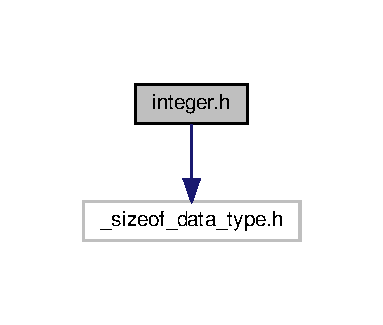
\includegraphics[width=194pt]{integer_8h__incl}
\end{center}
\end{figure}
\subsection*{Macros}
\begin{DoxyCompactItemize}
\item 
\mbox{\Hypertarget{integer_8h_aa401da1cbe54e588db88e13ed05308ae}\label{integer_8h_aa401da1cbe54e588db88e13ed05308ae}} 
\#define \hyperlink{integer_8h_aa401da1cbe54e588db88e13ed05308ae}{I\+N\+T8\+\_\+\+I\+S\+\_\+\+D\+E\+F\+I\+N\+ED}
\begin{DoxyCompactList}\small\item\em Flag to check whether 8 bit signed integer is defined. \end{DoxyCompactList}\item 
\mbox{\Hypertarget{integer_8h_adea19da0bf797e5de0354aab62b6a2c3}\label{integer_8h_adea19da0bf797e5de0354aab62b6a2c3}} 
\#define \hyperlink{integer_8h_adea19da0bf797e5de0354aab62b6a2c3}{U\+I\+N\+T8\+\_\+\+I\+S\+\_\+\+D\+E\+F\+I\+N\+ED}
\begin{DoxyCompactList}\small\item\em Flag to check whether 16 bit signed integer is defined. \end{DoxyCompactList}\item 
\mbox{\Hypertarget{integer_8h_a7a2c4d518e1638b47faa7c28c15f1989}\label{integer_8h_a7a2c4d518e1638b47faa7c28c15f1989}} 
\#define \hyperlink{integer_8h_a7a2c4d518e1638b47faa7c28c15f1989}{I\+N\+T16\+\_\+\+I\+S\+\_\+\+D\+E\+F\+I\+N\+ED}
\begin{DoxyCompactList}\small\item\em Flag to check whether 16 bit signed integer is defined. \end{DoxyCompactList}\item 
\mbox{\Hypertarget{integer_8h_a2a4a95fd69450b71295b5add4fc2a279}\label{integer_8h_a2a4a95fd69450b71295b5add4fc2a279}} 
\#define \hyperlink{integer_8h_a2a4a95fd69450b71295b5add4fc2a279}{U\+I\+N\+T16\+\_\+\+I\+S\+\_\+\+D\+E\+F\+I\+N\+ED}
\begin{DoxyCompactList}\small\item\em Flag to check whether 16 bit unsigned integer is defined. \end{DoxyCompactList}\item 
\mbox{\Hypertarget{integer_8h_a21fcd99088ee0c1e09ddc74877567fbb}\label{integer_8h_a21fcd99088ee0c1e09ddc74877567fbb}} 
\#define \hyperlink{integer_8h_a21fcd99088ee0c1e09ddc74877567fbb}{I\+N\+T32\+\_\+\+I\+S\+\_\+\+D\+E\+F\+I\+N\+ED}
\begin{DoxyCompactList}\small\item\em Flag to check whether 32 bit signed integer is defined. \end{DoxyCompactList}\item 
\mbox{\Hypertarget{integer_8h_a51c3b95a84e265395b18cc87052b677e}\label{integer_8h_a51c3b95a84e265395b18cc87052b677e}} 
\#define \hyperlink{integer_8h_a51c3b95a84e265395b18cc87052b677e}{U\+I\+N\+T32\+\_\+\+I\+S\+\_\+\+D\+E\+F\+I\+N\+ED}
\begin{DoxyCompactList}\small\item\em Flag to check whether 32 bit unsigned integer is defined. \end{DoxyCompactList}\item 
\mbox{\Hypertarget{integer_8h_a6058bc8df0e0b57d592ccd129dc1268d}\label{integer_8h_a6058bc8df0e0b57d592ccd129dc1268d}} 
\#define \hyperlink{integer_8h_a6058bc8df0e0b57d592ccd129dc1268d}{I\+N\+T64\+\_\+\+I\+S\+\_\+\+D\+E\+F\+I\+N\+ED}
\begin{DoxyCompactList}\small\item\em Flag to check whether 64 bit signed integer is defined. \end{DoxyCompactList}\item 
\mbox{\Hypertarget{integer_8h_abcee45b69494d6a1a7bc355d9bd26393}\label{integer_8h_abcee45b69494d6a1a7bc355d9bd26393}} 
\#define \hyperlink{integer_8h_abcee45b69494d6a1a7bc355d9bd26393}{U\+I\+N\+T64\+\_\+\+I\+S\+\_\+\+D\+E\+F\+I\+N\+ED}
\begin{DoxyCompactList}\small\item\em Flag to check whether 64 bit unsigned integer is defined. \end{DoxyCompactList}\end{DoxyCompactItemize}
\subsection*{Typedefs}
\begin{DoxyCompactItemize}
\item 
\mbox{\Hypertarget{integer_8h_a20c38cc5aac7cc6b0a3c6ab05428436d}\label{integer_8h_a20c38cc5aac7cc6b0a3c6ab05428436d}} 
typedef signed char \hyperlink{integer_8h_a20c38cc5aac7cc6b0a3c6ab05428436d}{int8\+\_\+t}
\begin{DoxyCompactList}\small\item\em 8 bit signed integer \end{DoxyCompactList}\item 
\mbox{\Hypertarget{integer_8h_ae1affc9ca37cfb624959c866a73f83c2}\label{integer_8h_ae1affc9ca37cfb624959c866a73f83c2}} 
typedef unsigned char \hyperlink{integer_8h_ae1affc9ca37cfb624959c866a73f83c2}{uint8\+\_\+t}
\begin{DoxyCompactList}\small\item\em 8 bit unsigned interger \end{DoxyCompactList}\item 
\mbox{\Hypertarget{integer_8h_a2140805d08462d474b82ddc8d1c2f3e6}\label{integer_8h_a2140805d08462d474b82ddc8d1c2f3e6}} 
typedef signed short \hyperlink{integer_8h_a2140805d08462d474b82ddc8d1c2f3e6}{int16\+\_\+t}
\begin{DoxyCompactList}\small\item\em 16 bit signed integer \end{DoxyCompactList}\item 
\mbox{\Hypertarget{integer_8h_a5a8b2dc9e45a9ee81a94ef304fb62505}\label{integer_8h_a5a8b2dc9e45a9ee81a94ef304fb62505}} 
typedef unsigned short \hyperlink{integer_8h_a5a8b2dc9e45a9ee81a94ef304fb62505}{uint16\+\_\+t}
\begin{DoxyCompactList}\small\item\em 16 bit unsigned integer \end{DoxyCompactList}\item 
\mbox{\Hypertarget{integer_8h_afd12020da5a235dfcf0c3c748fb5baed}\label{integer_8h_afd12020da5a235dfcf0c3c748fb5baed}} 
typedef signed long \hyperlink{integer_8h_afd12020da5a235dfcf0c3c748fb5baed}{int32\+\_\+t}
\begin{DoxyCompactList}\small\item\em 32 bit signed integer \end{DoxyCompactList}\item 
\mbox{\Hypertarget{integer_8h_a09a1e304d66d35dd47daffee9731edaa}\label{integer_8h_a09a1e304d66d35dd47daffee9731edaa}} 
typedef unsigned long \hyperlink{integer_8h_a09a1e304d66d35dd47daffee9731edaa}{uint32\+\_\+t}
\begin{DoxyCompactList}\small\item\em 32 bit unsigned integer \end{DoxyCompactList}\item 
\mbox{\Hypertarget{integer_8h_a21214d6ef664ff09b89c1fd75fe0a042}\label{integer_8h_a21214d6ef664ff09b89c1fd75fe0a042}} 
typedef signed long long \hyperlink{integer_8h_a21214d6ef664ff09b89c1fd75fe0a042}{int64\+\_\+t}
\begin{DoxyCompactList}\small\item\em 64 bit signed integer \end{DoxyCompactList}\item 
\mbox{\Hypertarget{integer_8h_a5dc34568a989dd90728a4ed499cd9fab}\label{integer_8h_a5dc34568a989dd90728a4ed499cd9fab}} 
typedef unsigned long long \hyperlink{integer_8h_a5dc34568a989dd90728a4ed499cd9fab}{uint64\+\_\+t}
\begin{DoxyCompactList}\small\item\em 64 bit unsigned integer \end{DoxyCompactList}\end{DoxyCompactItemize}


\subsection{Detailed Description}
Fixed-\/width integer type for C. 

\begin{DoxyAuthor}{Author}
Michelle Chen 
\end{DoxyAuthor}
\begin{DoxyCopyright}{Copyright}
M\+IT
\end{DoxyCopyright}
To use this header for C89 code, compile and run {\itshape get\+\_\+sizeof\+\_\+data\+\_\+type.\+c} to generate {\itshape \+\_\+sizeof\+\_\+data\+\_\+type.\+h}. {\itshape \hyperlink{integer_8h}{integer.\+h}} needs platform-\/specific data type information in {\itshape \+\_\+sizeof\+\_\+data\+\_\+type.\+h} to work properly.

This header is still experimental. Use it with caution. 
\hypertarget{platform_8h}{}\section{platform.\+h File Reference}
\label{platform_8h}\index{platform.\+h@{platform.\+h}}


Platform-\/specific data.  


\subsection*{Macros}
\begin{DoxyCompactItemize}
\item 
\#define \hyperlink{platform_8h_aa3d2b101ea5e31185ae18e499d30ed11}{E\+N\+D\+\_\+\+O\+F\+\_\+\+L\+I\+NE}~\char`\"{}\textbackslash{}n\char`\"{}
\begin{DoxyCompactList}\small\item\em End of line of specific host. \end{DoxyCompactList}\item 
\#define \hyperlink{platform_8h_af1e88bb4b1ff9546e6803eec85e0684c}{D\+I\+R\+E\+C\+T\+O\+R\+Y\+\_\+\+S\+E\+P\+A\+R\+A\+T\+OR}~\char`\"{}/\char`\"{}
\begin{DoxyCompactList}\small\item\em Directory separator of specific host. \end{DoxyCompactList}\item 
\#define \hyperlink{platform_8h_a532211c2f305b447fcfaf4b746756699}{S\+E\+A\+R\+C\+H\+\_\+\+P\+A\+T\+H\+\_\+\+S\+E\+P\+A\+R\+A\+T\+OR}~\char`\"{}\+:\char`\"{}
\begin{DoxyCompactList}\small\item\em Search path separator of specific host. \end{DoxyCompactList}\end{DoxyCompactItemize}


\subsection{Detailed Description}
Platform-\/specific data. 

\begin{DoxyAuthor}{Author}
Michelle Chen 
\end{DoxyAuthor}
\begin{DoxyCopyright}{Copyright}
M\+IT
\end{DoxyCopyright}
The macro definitions seen in this document represent the platform data of Unix. 

\subsection{Macro Definition Documentation}
\mbox{\Hypertarget{platform_8h_af1e88bb4b1ff9546e6803eec85e0684c}\label{platform_8h_af1e88bb4b1ff9546e6803eec85e0684c}} 
\index{platform.\+h@{platform.\+h}!D\+I\+R\+E\+C\+T\+O\+R\+Y\+\_\+\+S\+E\+P\+A\+R\+A\+T\+OR@{D\+I\+R\+E\+C\+T\+O\+R\+Y\+\_\+\+S\+E\+P\+A\+R\+A\+T\+OR}}
\index{D\+I\+R\+E\+C\+T\+O\+R\+Y\+\_\+\+S\+E\+P\+A\+R\+A\+T\+OR@{D\+I\+R\+E\+C\+T\+O\+R\+Y\+\_\+\+S\+E\+P\+A\+R\+A\+T\+OR}!platform.\+h@{platform.\+h}}
\subsubsection{\texorpdfstring{D\+I\+R\+E\+C\+T\+O\+R\+Y\+\_\+\+S\+E\+P\+A\+R\+A\+T\+OR}{DIRECTORY\_SEPARATOR}}
{\footnotesize\ttfamily \#define D\+I\+R\+E\+C\+T\+O\+R\+Y\+\_\+\+S\+E\+P\+A\+R\+A\+T\+OR~\char`\"{}/\char`\"{}}



Directory separator of specific host. 

Currently, D\+I\+R\+E\+C\+T\+O\+R\+Y\+\_\+\+S\+E\+P\+A\+R\+A\+T\+OR works on Windows and Unix. \mbox{\Hypertarget{platform_8h_aa3d2b101ea5e31185ae18e499d30ed11}\label{platform_8h_aa3d2b101ea5e31185ae18e499d30ed11}} 
\index{platform.\+h@{platform.\+h}!E\+N\+D\+\_\+\+O\+F\+\_\+\+L\+I\+NE@{E\+N\+D\+\_\+\+O\+F\+\_\+\+L\+I\+NE}}
\index{E\+N\+D\+\_\+\+O\+F\+\_\+\+L\+I\+NE@{E\+N\+D\+\_\+\+O\+F\+\_\+\+L\+I\+NE}!platform.\+h@{platform.\+h}}
\subsubsection{\texorpdfstring{E\+N\+D\+\_\+\+O\+F\+\_\+\+L\+I\+NE}{END\_OF\_LINE}}
{\footnotesize\ttfamily \#define E\+N\+D\+\_\+\+O\+F\+\_\+\+L\+I\+NE~\char`\"{}\textbackslash{}n\char`\"{}}



End of line of specific host. 

C will handle platform-\/specific end of line automatically. Hence, we always set E\+N\+D\+\_\+\+O\+F\+\_\+\+L\+I\+NE the same value. \mbox{\Hypertarget{platform_8h_a532211c2f305b447fcfaf4b746756699}\label{platform_8h_a532211c2f305b447fcfaf4b746756699}} 
\index{platform.\+h@{platform.\+h}!S\+E\+A\+R\+C\+H\+\_\+\+P\+A\+T\+H\+\_\+\+S\+E\+P\+A\+R\+A\+T\+OR@{S\+E\+A\+R\+C\+H\+\_\+\+P\+A\+T\+H\+\_\+\+S\+E\+P\+A\+R\+A\+T\+OR}}
\index{S\+E\+A\+R\+C\+H\+\_\+\+P\+A\+T\+H\+\_\+\+S\+E\+P\+A\+R\+A\+T\+OR@{S\+E\+A\+R\+C\+H\+\_\+\+P\+A\+T\+H\+\_\+\+S\+E\+P\+A\+R\+A\+T\+OR}!platform.\+h@{platform.\+h}}
\subsubsection{\texorpdfstring{S\+E\+A\+R\+C\+H\+\_\+\+P\+A\+T\+H\+\_\+\+S\+E\+P\+A\+R\+A\+T\+OR}{SEARCH\_PATH\_SEPARATOR}}
{\footnotesize\ttfamily \#define S\+E\+A\+R\+C\+H\+\_\+\+P\+A\+T\+H\+\_\+\+S\+E\+P\+A\+R\+A\+T\+OR~\char`\"{}\+:\char`\"{}}



Search path separator of specific host. 

Currently, S\+E\+A\+R\+C\+H\+\_\+\+P\+A\+T\+H\+\_\+\+S\+E\+P\+A\+R\+A\+T\+OR works on Windows and Unix. 
\hypertarget{print_8h}{}\section{print.\+h File Reference}
\label{print_8h}\index{print.\+h@{print.\+h}}


Console printing related macros.  


{\ttfamily \#include $<$stdio.\+h$>$}\newline
Include dependency graph for print.\+h\+:\nopagebreak
\begin{figure}[H]
\begin{center}
\leavevmode
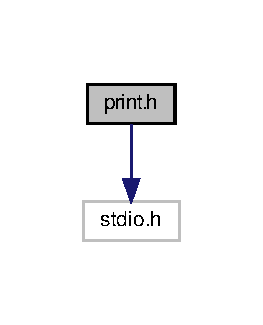
\includegraphics[width=125pt]{print_8h__incl}
\end{center}
\end{figure}
\subsection*{Macros}
\begin{DoxyCompactItemize}
\item 
\mbox{\Hypertarget{print_8h_aa3d2b101ea5e31185ae18e499d30ed11}\label{print_8h_aa3d2b101ea5e31185ae18e499d30ed11}} 
\#define {\bfseries E\+N\+D\+\_\+\+O\+F\+\_\+\+L\+I\+NE}~\char`\"{}\textbackslash{}n\char`\"{}
\item 
\#define \hyperlink{print_8h_af990e936c83edcff058ae8ec5864adec}{P\+R\+I\+NT}(format, ...)
\begin{DoxyCompactList}\small\item\em Print formated string to {\bfseries stdout} without trailing E\+OL. \end{DoxyCompactList}\item 
\#define \hyperlink{print_8h_a36f6a6453e7533808c32a37f455068a0}{P\+E\+R\+R\+OR}(format, ...)
\begin{DoxyCompactList}\small\item\em Print formated string to {\bfseries stderr} without trailing E\+OL. \end{DoxyCompactList}\item 
\#define \hyperlink{print_8h_ad5ec9098821844c0c27cd849fc930c90}{P\+U\+TS}(format, ...)
\begin{DoxyCompactList}\small\item\em Print formated string to {\bfseries stdout} with trailing E\+OL. \end{DoxyCompactList}\item 
\#define \hyperlink{print_8h_a84559fc324a4622242ee818f9025141f}{P\+U\+T\+E\+RR}(format, ...)
\begin{DoxyCompactList}\small\item\em Print formated string to {\bfseries stderr} with trailing E\+OL. \end{DoxyCompactList}\item 
\#define \hyperlink{print_8h_a994994514490b70ee6a5dd679f28acbc}{D\+E\+B\+U\+G\+\_\+\+I\+N\+FO}(format, ...)
\begin{DoxyCompactList}\small\item\em Print formated debug message to {\bfseries stderr} with trailing E\+OL. \end{DoxyCompactList}\end{DoxyCompactItemize}


\subsection{Detailed Description}
Console printing related macros. 

\begin{DoxyAuthor}{Author}
Michael Chen 
\end{DoxyAuthor}
\begin{DoxyCopyright}{Copyright}
M\+IT
\end{DoxyCopyright}
The macro definition seen in this document represent the platform data of Unix. 

\subsection{Macro Definition Documentation}
\mbox{\Hypertarget{print_8h_a994994514490b70ee6a5dd679f28acbc}\label{print_8h_a994994514490b70ee6a5dd679f28acbc}} 
\index{print.\+h@{print.\+h}!D\+E\+B\+U\+G\+\_\+\+I\+N\+FO@{D\+E\+B\+U\+G\+\_\+\+I\+N\+FO}}
\index{D\+E\+B\+U\+G\+\_\+\+I\+N\+FO@{D\+E\+B\+U\+G\+\_\+\+I\+N\+FO}!print.\+h@{print.\+h}}
\subsubsection{\texorpdfstring{D\+E\+B\+U\+G\+\_\+\+I\+N\+FO}{DEBUG\_INFO}}
{\footnotesize\ttfamily \#define D\+E\+B\+U\+G\+\_\+\+I\+N\+FO(\begin{DoxyParamCaption}\item[{}]{format,  }\item[{}]{... }\end{DoxyParamCaption})}

{\bfseries Value\+:}
\begin{DoxyCode}
\{ \(\backslash\)
        fprintf(stderr, \textcolor{stringliteral}{"(%s:%d) "} format \textcolor{stringliteral}{"%s"}, \(\backslash\)
            \_\_FILE\_\_, \_\_LINE\_\_, ##\_\_VA\_ARGS\_\_, \hyperlink{platform_8h_aa3d2b101ea5e31185ae18e499d30ed11}{END\_OF\_LINE}); \(\backslash\)
    \}
\end{DoxyCode}


Print formated debug message to {\bfseries stderr} with trailing E\+OL. 

{\bfseries D\+E\+B\+U\+G\+\_\+\+I\+N\+FO} works similarly to {\bfseries P\+U\+T\+E\+RR} but adds source file and line number. Hence, developers can track the location of the message more easily. \mbox{\Hypertarget{print_8h_a36f6a6453e7533808c32a37f455068a0}\label{print_8h_a36f6a6453e7533808c32a37f455068a0}} 
\index{print.\+h@{print.\+h}!P\+E\+R\+R\+OR@{P\+E\+R\+R\+OR}}
\index{P\+E\+R\+R\+OR@{P\+E\+R\+R\+OR}!print.\+h@{print.\+h}}
\subsubsection{\texorpdfstring{P\+E\+R\+R\+OR}{PERROR}}
{\footnotesize\ttfamily \#define P\+E\+R\+R\+OR(\begin{DoxyParamCaption}\item[{}]{format,  }\item[{}]{... }\end{DoxyParamCaption})}

{\bfseries Value\+:}
\begin{DoxyCode}
\{ \(\backslash\)
        fprintf(stderr, format, ##\_\_VA\_ARGS\_\_); \(\backslash\)
    \}
\end{DoxyCode}


Print formated string to {\bfseries stderr} without trailing E\+OL. 

{\bfseries P\+E\+R\+R\+OR} works as {\bfseries P\+R\+I\+NT}, but to {\bfseries stderr}. \mbox{\Hypertarget{print_8h_af990e936c83edcff058ae8ec5864adec}\label{print_8h_af990e936c83edcff058ae8ec5864adec}} 
\index{print.\+h@{print.\+h}!P\+R\+I\+NT@{P\+R\+I\+NT}}
\index{P\+R\+I\+NT@{P\+R\+I\+NT}!print.\+h@{print.\+h}}
\subsubsection{\texorpdfstring{P\+R\+I\+NT}{PRINT}}
{\footnotesize\ttfamily \#define P\+R\+I\+NT(\begin{DoxyParamCaption}\item[{}]{format,  }\item[{}]{... }\end{DoxyParamCaption})}

{\bfseries Value\+:}
\begin{DoxyCode}
\{ \(\backslash\)
        fprintf(stdout, format, ##\_\_VA\_ARGS\_\_); \(\backslash\)
    \}
\end{DoxyCode}


Print formated string to {\bfseries stdout} without trailing E\+OL. 

Basically, {\bfseries P\+R\+I\+NT} is just a repackaged {\itshape printf} function seen {\bfseries stdio.\+h}. \mbox{\Hypertarget{print_8h_a84559fc324a4622242ee818f9025141f}\label{print_8h_a84559fc324a4622242ee818f9025141f}} 
\index{print.\+h@{print.\+h}!P\+U\+T\+E\+RR@{P\+U\+T\+E\+RR}}
\index{P\+U\+T\+E\+RR@{P\+U\+T\+E\+RR}!print.\+h@{print.\+h}}
\subsubsection{\texorpdfstring{P\+U\+T\+E\+RR}{PUTERR}}
{\footnotesize\ttfamily \#define P\+U\+T\+E\+RR(\begin{DoxyParamCaption}\item[{}]{format,  }\item[{}]{... }\end{DoxyParamCaption})}

{\bfseries Value\+:}
\begin{DoxyCode}
\{ \(\backslash\)
        fprintf(stderr, format \textcolor{stringliteral}{"%s"}, ##\_\_VA\_ARGS\_\_, \hyperlink{platform_8h_aa3d2b101ea5e31185ae18e499d30ed11}{END\_OF\_LINE}); \(\backslash\)
    \}
\end{DoxyCode}


Print formated string to {\bfseries stderr} with trailing E\+OL. 

The E\+OL will change according to the host environment. \mbox{\Hypertarget{print_8h_ad5ec9098821844c0c27cd849fc930c90}\label{print_8h_ad5ec9098821844c0c27cd849fc930c90}} 
\index{print.\+h@{print.\+h}!P\+U\+TS@{P\+U\+TS}}
\index{P\+U\+TS@{P\+U\+TS}!print.\+h@{print.\+h}}
\subsubsection{\texorpdfstring{P\+U\+TS}{PUTS}}
{\footnotesize\ttfamily \#define P\+U\+TS(\begin{DoxyParamCaption}\item[{}]{format,  }\item[{}]{... }\end{DoxyParamCaption})}

{\bfseries Value\+:}
\begin{DoxyCode}
\{ \(\backslash\)
        fprintf(stdout, format \textcolor{stringliteral}{"%s"}, ##\_\_VA\_ARGS\_\_, \hyperlink{platform_8h_aa3d2b101ea5e31185ae18e499d30ed11}{END\_OF\_LINE}); \(\backslash\)
    \}
\end{DoxyCode}


Print formated string to {\bfseries stdout} with trailing E\+OL. 

The E\+OL will change according to the host environment. 
\hypertarget{term__color_8h}{}\section{term\+\_\+color.\+h File Reference}
\label{term__color_8h}\index{term\+\_\+color.\+h@{term\+\_\+color.\+h}}


Add colors, either foreground or background, on console environment.  


\subsection*{Macros}
\begin{DoxyCompactItemize}
\item 
\mbox{\Hypertarget{term__color_8h_a1b44aa6933d2aba22a724787032ffb49}\label{term__color_8h_a1b44aa6933d2aba22a724787032ffb49}} 
\#define {\bfseries \+\_\+\+T\+E\+R\+M\+\_\+\+C\+O\+L\+O\+R\+\_\+\+D\+E\+F\+I\+N\+ED}
\item 
\mbox{\Hypertarget{term__color_8h_a5d08f00bc9bcef4f7cecd3467addf42b}\label{term__color_8h_a5d08f00bc9bcef4f7cecd3467addf42b}} 
\#define \hyperlink{term__color_8h_a5d08f00bc9bcef4f7cecd3467addf42b}{T\+E\+R\+M\+\_\+\+C\+O\+L\+O\+R\+\_\+\+R\+E\+S\+ET}~\char`\"{}\textbackslash{}e\mbox{[}0m\char`\"{}
\begin{DoxyCompactList}\small\item\em Reset console color. \end{DoxyCompactList}\item 
\mbox{\Hypertarget{term__color_8h_ad2e838c3c191be13ff1b47fda72f1f22}\label{term__color_8h_ad2e838c3c191be13ff1b47fda72f1f22}} 
\#define \hyperlink{term__color_8h_ad2e838c3c191be13ff1b47fda72f1f22}{T\+E\+R\+M\+\_\+\+C\+O\+L\+O\+R\+\_\+\+B\+L\+A\+CK}~\char`\"{}\textbackslash{}e\mbox{[}0;30m\char`\"{}
\begin{DoxyCompactList}\small\item\em Regular black color in foreground. \end{DoxyCompactList}\item 
\mbox{\Hypertarget{term__color_8h_a149966c2d8deae14337743cc86213686}\label{term__color_8h_a149966c2d8deae14337743cc86213686}} 
\#define \hyperlink{term__color_8h_a149966c2d8deae14337743cc86213686}{T\+E\+R\+M\+\_\+\+C\+O\+L\+O\+R\+\_\+\+R\+ED}~\char`\"{}\textbackslash{}e\mbox{[}0;31m\char`\"{}
\begin{DoxyCompactList}\small\item\em Regular red color in foreground. \end{DoxyCompactList}\item 
\mbox{\Hypertarget{term__color_8h_a684eca9ff18601657c590e87c04d3003}\label{term__color_8h_a684eca9ff18601657c590e87c04d3003}} 
\#define \hyperlink{term__color_8h_a684eca9ff18601657c590e87c04d3003}{T\+E\+R\+M\+\_\+\+C\+O\+L\+O\+R\+\_\+\+G\+R\+E\+EN}~\char`\"{}\textbackslash{}e\mbox{[}0;32m\char`\"{}
\begin{DoxyCompactList}\small\item\em Regular green color in foreground. \end{DoxyCompactList}\item 
\mbox{\Hypertarget{term__color_8h_a50fd646705ee1bf7e4496302acfd8a94}\label{term__color_8h_a50fd646705ee1bf7e4496302acfd8a94}} 
\#define \hyperlink{term__color_8h_a50fd646705ee1bf7e4496302acfd8a94}{T\+E\+R\+M\+\_\+\+C\+O\+L\+O\+R\+\_\+\+Y\+E\+L\+L\+OW}~\char`\"{}\textbackslash{}e\mbox{[}0;33m\char`\"{}
\begin{DoxyCompactList}\small\item\em Regular yellow color in foreground. \end{DoxyCompactList}\item 
\mbox{\Hypertarget{term__color_8h_a403697ea12f3cb2dd5b0051efaa00a8d}\label{term__color_8h_a403697ea12f3cb2dd5b0051efaa00a8d}} 
\#define \hyperlink{term__color_8h_a403697ea12f3cb2dd5b0051efaa00a8d}{T\+E\+R\+M\+\_\+\+C\+O\+L\+O\+R\+\_\+\+B\+L\+UE}~\char`\"{}\textbackslash{}e\mbox{[}0;34m\char`\"{}
\begin{DoxyCompactList}\small\item\em Regular blue color in foreground. \end{DoxyCompactList}\item 
\mbox{\Hypertarget{term__color_8h_a954de58d7b12304297d694bc352b48a3}\label{term__color_8h_a954de58d7b12304297d694bc352b48a3}} 
\#define \hyperlink{term__color_8h_a954de58d7b12304297d694bc352b48a3}{T\+E\+R\+M\+\_\+\+C\+O\+L\+O\+R\+\_\+\+P\+U\+R\+P\+LE}~\char`\"{}\textbackslash{}e\mbox{[}0;35m\char`\"{}
\begin{DoxyCompactList}\small\item\em Regular purple color in foreground. \end{DoxyCompactList}\item 
\mbox{\Hypertarget{term__color_8h_afcc94812f2fbb0b4c388642e2825065a}\label{term__color_8h_afcc94812f2fbb0b4c388642e2825065a}} 
\#define \hyperlink{term__color_8h_afcc94812f2fbb0b4c388642e2825065a}{T\+E\+R\+M\+\_\+\+C\+O\+L\+O\+R\+\_\+\+C\+Y\+AN}~\char`\"{}\textbackslash{}e\mbox{[}0;36m\char`\"{}
\begin{DoxyCompactList}\small\item\em Regular cyan color in foreground. \end{DoxyCompactList}\item 
\mbox{\Hypertarget{term__color_8h_aab6765d472f7ad6a69ac4ad24ba2cad4}\label{term__color_8h_aab6765d472f7ad6a69ac4ad24ba2cad4}} 
\#define \hyperlink{term__color_8h_aab6765d472f7ad6a69ac4ad24ba2cad4}{T\+E\+R\+M\+\_\+\+C\+O\+L\+O\+R\+\_\+\+W\+H\+I\+TE}~\char`\"{}\textbackslash{}e\mbox{[}0;37m\char`\"{}
\begin{DoxyCompactList}\small\item\em Regular white color in foreground. \end{DoxyCompactList}\item 
\mbox{\Hypertarget{term__color_8h_ad1d828e289cab37976224793f021bf49}\label{term__color_8h_ad1d828e289cab37976224793f021bf49}} 
\#define \hyperlink{term__color_8h_ad1d828e289cab37976224793f021bf49}{T\+E\+R\+M\+\_\+\+B\+R\+I\+G\+H\+T\+\_\+\+C\+O\+L\+O\+R\+\_\+\+B\+L\+A\+CK}~\char`\"{}\textbackslash{}e\mbox{[}0;90m\char`\"{}
\begin{DoxyCompactList}\small\item\em Bright black color in foreground. \end{DoxyCompactList}\item 
\mbox{\Hypertarget{term__color_8h_aa7cc7ec53eaaa16dcfce622b5420b241}\label{term__color_8h_aa7cc7ec53eaaa16dcfce622b5420b241}} 
\#define \hyperlink{term__color_8h_aa7cc7ec53eaaa16dcfce622b5420b241}{T\+E\+R\+M\+\_\+\+B\+R\+I\+G\+H\+T\+\_\+\+C\+O\+L\+O\+R\+\_\+\+R\+ED}~\char`\"{}\textbackslash{}e\mbox{[}0;91m\char`\"{}
\begin{DoxyCompactList}\small\item\em Bright red color in foreground. \end{DoxyCompactList}\item 
\mbox{\Hypertarget{term__color_8h_a2ed22b24d193cf6e0b77f4fedfaadad6}\label{term__color_8h_a2ed22b24d193cf6e0b77f4fedfaadad6}} 
\#define \hyperlink{term__color_8h_a2ed22b24d193cf6e0b77f4fedfaadad6}{T\+E\+R\+M\+\_\+\+B\+R\+I\+G\+H\+T\+\_\+\+C\+O\+L\+O\+R\+\_\+\+G\+R\+E\+EN}~\char`\"{}\textbackslash{}e\mbox{[}0;92m\char`\"{}
\begin{DoxyCompactList}\small\item\em Bright green color in foreground. \end{DoxyCompactList}\item 
\mbox{\Hypertarget{term__color_8h_a59e454f5dab1dfb69ce12cb745e4c99d}\label{term__color_8h_a59e454f5dab1dfb69ce12cb745e4c99d}} 
\#define \hyperlink{term__color_8h_a59e454f5dab1dfb69ce12cb745e4c99d}{T\+E\+R\+M\+\_\+\+B\+R\+I\+G\+H\+T\+\_\+\+C\+O\+L\+O\+R\+\_\+\+Y\+E\+L\+L\+OW}~\char`\"{}\textbackslash{}e\mbox{[}0;93m\char`\"{}
\begin{DoxyCompactList}\small\item\em Bright yellow color in foreground. \end{DoxyCompactList}\item 
\mbox{\Hypertarget{term__color_8h_a9a45e0bc5124cb4cb1f95b229b6f847e}\label{term__color_8h_a9a45e0bc5124cb4cb1f95b229b6f847e}} 
\#define \hyperlink{term__color_8h_a9a45e0bc5124cb4cb1f95b229b6f847e}{T\+E\+R\+M\+\_\+\+B\+R\+I\+G\+H\+T\+\_\+\+C\+O\+L\+O\+R\+\_\+\+B\+L\+UE}~\char`\"{}\textbackslash{}e\mbox{[}0;94m\char`\"{}
\begin{DoxyCompactList}\small\item\em Bright blue color in foreground. \end{DoxyCompactList}\item 
\mbox{\Hypertarget{term__color_8h_adfef88b8796fe5dab6f01784713afdfd}\label{term__color_8h_adfef88b8796fe5dab6f01784713afdfd}} 
\#define \hyperlink{term__color_8h_adfef88b8796fe5dab6f01784713afdfd}{T\+E\+R\+M\+\_\+\+B\+R\+I\+G\+H\+T\+\_\+\+C\+O\+L\+O\+R\+\_\+\+P\+U\+R\+P\+LE}~\char`\"{}\textbackslash{}e\mbox{[}0;95m\char`\"{}
\begin{DoxyCompactList}\small\item\em Bright purple color in foreground. \end{DoxyCompactList}\item 
\mbox{\Hypertarget{term__color_8h_a68e7e1fd8b1a7e777c13a41e1ddb1c05}\label{term__color_8h_a68e7e1fd8b1a7e777c13a41e1ddb1c05}} 
\#define \hyperlink{term__color_8h_a68e7e1fd8b1a7e777c13a41e1ddb1c05}{T\+E\+R\+M\+\_\+\+B\+R\+I\+G\+H\+T\+\_\+\+C\+O\+L\+O\+R\+\_\+\+C\+Y\+AN}~\char`\"{}\textbackslash{}e\mbox{[}0;96m\char`\"{}
\begin{DoxyCompactList}\small\item\em Bright cyan color in foreground. \end{DoxyCompactList}\item 
\mbox{\Hypertarget{term__color_8h_a64fb2f0ff9c4d5b30f0e76eeef0f5eb9}\label{term__color_8h_a64fb2f0ff9c4d5b30f0e76eeef0f5eb9}} 
\#define \hyperlink{term__color_8h_a64fb2f0ff9c4d5b30f0e76eeef0f5eb9}{T\+E\+R\+M\+\_\+\+B\+R\+I\+G\+H\+T\+\_\+\+C\+O\+L\+O\+R\+\_\+\+W\+H\+I\+TE}~\char`\"{}\textbackslash{}e\mbox{[}0;97m\char`\"{}
\begin{DoxyCompactList}\small\item\em Bright white color in foreground. \end{DoxyCompactList}\item 
\mbox{\Hypertarget{term__color_8h_a2c4cea161da44626b24a5df3d7bbddae}\label{term__color_8h_a2c4cea161da44626b24a5df3d7bbddae}} 
\#define \hyperlink{term__color_8h_a2c4cea161da44626b24a5df3d7bbddae}{T\+E\+R\+M\+\_\+\+B\+O\+L\+D\+\_\+\+C\+O\+L\+O\+R\+\_\+\+B\+L\+A\+CK}~\char`\"{}\textbackslash{}e\mbox{[}1;30m\char`\"{}
\begin{DoxyCompactList}\small\item\em Bold black color in foreground. \end{DoxyCompactList}\item 
\mbox{\Hypertarget{term__color_8h_a83bda39c53766a016eb46b80a0986b33}\label{term__color_8h_a83bda39c53766a016eb46b80a0986b33}} 
\#define \hyperlink{term__color_8h_a83bda39c53766a016eb46b80a0986b33}{T\+E\+R\+M\+\_\+\+B\+O\+L\+D\+\_\+\+C\+O\+L\+O\+R\+\_\+\+R\+ED}~\char`\"{}\textbackslash{}e\mbox{[}1;31m\char`\"{}
\begin{DoxyCompactList}\small\item\em Bold red color in foreground. \end{DoxyCompactList}\item 
\mbox{\Hypertarget{term__color_8h_a2fe48e1e58b00588443cc79c9d196081}\label{term__color_8h_a2fe48e1e58b00588443cc79c9d196081}} 
\#define \hyperlink{term__color_8h_a2fe48e1e58b00588443cc79c9d196081}{T\+E\+R\+M\+\_\+\+B\+O\+L\+D\+\_\+\+C\+O\+L\+O\+R\+\_\+\+G\+R\+E\+EN}~\char`\"{}\textbackslash{}e\mbox{[}1;32m\char`\"{}
\begin{DoxyCompactList}\small\item\em Bold green color in foreground. \end{DoxyCompactList}\item 
\mbox{\Hypertarget{term__color_8h_a8ac4240303ef04cee82b6b6bf21deb4c}\label{term__color_8h_a8ac4240303ef04cee82b6b6bf21deb4c}} 
\#define \hyperlink{term__color_8h_a8ac4240303ef04cee82b6b6bf21deb4c}{T\+E\+R\+M\+\_\+\+B\+O\+L\+D\+\_\+\+C\+O\+L\+O\+R\+\_\+\+Y\+E\+L\+L\+OW}~\char`\"{}\textbackslash{}e\mbox{[}1;33m\char`\"{}
\begin{DoxyCompactList}\small\item\em Bold yellow color in foreground. \end{DoxyCompactList}\item 
\mbox{\Hypertarget{term__color_8h_adbe32193ef5bf2e2b79ce2f618811df8}\label{term__color_8h_adbe32193ef5bf2e2b79ce2f618811df8}} 
\#define \hyperlink{term__color_8h_adbe32193ef5bf2e2b79ce2f618811df8}{T\+E\+R\+M\+\_\+\+B\+O\+L\+D\+\_\+\+C\+O\+L\+O\+R\+\_\+\+B\+L\+UE}~\char`\"{}\textbackslash{}e\mbox{[}1;34m\char`\"{}
\begin{DoxyCompactList}\small\item\em Bold blue color in foreground. \end{DoxyCompactList}\item 
\mbox{\Hypertarget{term__color_8h_a1344218bfbbd910e2ff67ce98428b154}\label{term__color_8h_a1344218bfbbd910e2ff67ce98428b154}} 
\#define \hyperlink{term__color_8h_a1344218bfbbd910e2ff67ce98428b154}{T\+E\+R\+M\+\_\+\+B\+O\+L\+D\+\_\+\+C\+O\+L\+O\+R\+\_\+\+P\+U\+R\+P\+LE}~\char`\"{}\textbackslash{}e\mbox{[}1;35m\char`\"{}
\begin{DoxyCompactList}\small\item\em Bold purple color in foreground. \end{DoxyCompactList}\item 
\mbox{\Hypertarget{term__color_8h_a743c12e30f6341ba23f32cef97921bc0}\label{term__color_8h_a743c12e30f6341ba23f32cef97921bc0}} 
\#define \hyperlink{term__color_8h_a743c12e30f6341ba23f32cef97921bc0}{T\+E\+R\+M\+\_\+\+B\+O\+L\+D\+\_\+\+C\+O\+L\+O\+R\+\_\+\+C\+Y\+AN}~\char`\"{}\textbackslash{}e\mbox{[}1;36m\char`\"{}
\begin{DoxyCompactList}\small\item\em Bold cyan color in foreground. \end{DoxyCompactList}\item 
\mbox{\Hypertarget{term__color_8h_a17e274c247808139c3de6d313cf12714}\label{term__color_8h_a17e274c247808139c3de6d313cf12714}} 
\#define \hyperlink{term__color_8h_a17e274c247808139c3de6d313cf12714}{T\+E\+R\+M\+\_\+\+B\+O\+L\+D\+\_\+\+C\+O\+L\+O\+R\+\_\+\+W\+H\+I\+TE}~\char`\"{}\textbackslash{}e\mbox{[}1;37m\char`\"{}
\begin{DoxyCompactList}\small\item\em Bold white color in foreground. \end{DoxyCompactList}\item 
\mbox{\Hypertarget{term__color_8h_a150d30e59774da6022a8121a5fbed709}\label{term__color_8h_a150d30e59774da6022a8121a5fbed709}} 
\#define \hyperlink{term__color_8h_a150d30e59774da6022a8121a5fbed709}{T\+E\+R\+M\+\_\+\+B\+O\+L\+D\+\_\+\+B\+R\+I\+G\+H\+T\+\_\+\+C\+O\+L\+O\+R\+\_\+\+B\+L\+A\+CK}~\char`\"{}\textbackslash{}e\mbox{[}1;90m\char`\"{}
\begin{DoxyCompactList}\small\item\em Bold bright black color in foreground. \end{DoxyCompactList}\item 
\mbox{\Hypertarget{term__color_8h_a31b390595cf240f411a99ea0a3763c4b}\label{term__color_8h_a31b390595cf240f411a99ea0a3763c4b}} 
\#define \hyperlink{term__color_8h_a31b390595cf240f411a99ea0a3763c4b}{T\+E\+R\+M\+\_\+\+B\+O\+L\+D\+\_\+\+B\+R\+I\+G\+H\+T\+\_\+\+C\+O\+L\+O\+R\+\_\+\+R\+ED}~\char`\"{}\textbackslash{}e\mbox{[}1;91m\char`\"{}
\begin{DoxyCompactList}\small\item\em Bold bright red color in foreground. \end{DoxyCompactList}\item 
\mbox{\Hypertarget{term__color_8h_a7cf85190f3b32562dce94bbeb0501217}\label{term__color_8h_a7cf85190f3b32562dce94bbeb0501217}} 
\#define \hyperlink{term__color_8h_a7cf85190f3b32562dce94bbeb0501217}{T\+E\+R\+M\+\_\+\+B\+O\+L\+D\+\_\+\+B\+R\+I\+G\+H\+T\+\_\+\+C\+O\+L\+O\+R\+\_\+\+G\+R\+E\+EN}~\char`\"{}\textbackslash{}e\mbox{[}1;92m\char`\"{}
\begin{DoxyCompactList}\small\item\em Bold bright green color in foreground. \end{DoxyCompactList}\item 
\mbox{\Hypertarget{term__color_8h_a7f9c65e5e72d52c4885492c30d9a5e58}\label{term__color_8h_a7f9c65e5e72d52c4885492c30d9a5e58}} 
\#define \hyperlink{term__color_8h_a7f9c65e5e72d52c4885492c30d9a5e58}{T\+E\+R\+M\+\_\+\+B\+O\+L\+D\+\_\+\+B\+R\+I\+G\+H\+T\+\_\+\+C\+O\+L\+O\+R\+\_\+\+Y\+E\+L\+L\+OW}~\char`\"{}\textbackslash{}e\mbox{[}1;93m\char`\"{}
\begin{DoxyCompactList}\small\item\em Bold bright yellow color in foreground. \end{DoxyCompactList}\item 
\mbox{\Hypertarget{term__color_8h_ad193c2b1cc24884228169aeed6901510}\label{term__color_8h_ad193c2b1cc24884228169aeed6901510}} 
\#define \hyperlink{term__color_8h_ad193c2b1cc24884228169aeed6901510}{T\+E\+R\+M\+\_\+\+B\+O\+L\+D\+\_\+\+B\+R\+I\+G\+H\+T\+\_\+\+C\+O\+L\+O\+R\+\_\+\+B\+L\+UE}~\char`\"{}\textbackslash{}e\mbox{[}1;94m\char`\"{}
\begin{DoxyCompactList}\small\item\em Bold bright blue color in foreground. \end{DoxyCompactList}\item 
\mbox{\Hypertarget{term__color_8h_a2f310cf432bcec4e1a3339da2f362edb}\label{term__color_8h_a2f310cf432bcec4e1a3339da2f362edb}} 
\#define \hyperlink{term__color_8h_a2f310cf432bcec4e1a3339da2f362edb}{T\+E\+R\+M\+\_\+\+B\+O\+L\+D\+\_\+\+B\+R\+I\+G\+H\+T\+\_\+\+C\+O\+L\+O\+R\+\_\+\+P\+U\+R\+P\+LE}~\char`\"{}\textbackslash{}e\mbox{[}1;95m\char`\"{}
\begin{DoxyCompactList}\small\item\em Bold bright purple color in foreground. \end{DoxyCompactList}\item 
\mbox{\Hypertarget{term__color_8h_af90c0c7177ebc403cd6c87f5d002420d}\label{term__color_8h_af90c0c7177ebc403cd6c87f5d002420d}} 
\#define \hyperlink{term__color_8h_af90c0c7177ebc403cd6c87f5d002420d}{T\+E\+R\+M\+\_\+\+B\+O\+L\+D\+\_\+\+B\+R\+I\+G\+H\+T\+\_\+\+C\+O\+L\+O\+R\+\_\+\+C\+Y\+AN}~\char`\"{}\textbackslash{}e\mbox{[}1;96m\char`\"{}
\begin{DoxyCompactList}\small\item\em Bold bright cyan color in foreground. \end{DoxyCompactList}\item 
\mbox{\Hypertarget{term__color_8h_a257993cee3981b3e99dd9be943845b19}\label{term__color_8h_a257993cee3981b3e99dd9be943845b19}} 
\#define \hyperlink{term__color_8h_a257993cee3981b3e99dd9be943845b19}{T\+E\+R\+M\+\_\+\+B\+O\+L\+D\+\_\+\+B\+R\+I\+G\+H\+T\+\_\+\+C\+O\+L\+O\+R\+\_\+\+W\+H\+I\+TE}~\char`\"{}\textbackslash{}e\mbox{[}1;97m\char`\"{}
\begin{DoxyCompactList}\small\item\em Bold bright white color in foreground. \end{DoxyCompactList}\item 
\mbox{\Hypertarget{term__color_8h_afb61486725dabf524b49340c8490fb12}\label{term__color_8h_afb61486725dabf524b49340c8490fb12}} 
\#define \hyperlink{term__color_8h_afb61486725dabf524b49340c8490fb12}{T\+E\+R\+M\+\_\+\+U\+N\+D\+E\+R\+L\+I\+N\+E\+\_\+\+C\+O\+L\+O\+R\+\_\+\+B\+L\+A\+CK}~\char`\"{}\textbackslash{}e\mbox{[}4;30m\char`\"{}
\begin{DoxyCompactList}\small\item\em Underline black color in foreground. \end{DoxyCompactList}\item 
\mbox{\Hypertarget{term__color_8h_aacb10ec64746332aed4cc4ae4336b39a}\label{term__color_8h_aacb10ec64746332aed4cc4ae4336b39a}} 
\#define \hyperlink{term__color_8h_aacb10ec64746332aed4cc4ae4336b39a}{T\+E\+R\+M\+\_\+\+U\+N\+D\+E\+R\+L\+I\+N\+E\+\_\+\+C\+O\+L\+O\+R\+\_\+\+R\+ED}~\char`\"{}\textbackslash{}e\mbox{[}4;31m\char`\"{}
\begin{DoxyCompactList}\small\item\em Underline red color in foreground. \end{DoxyCompactList}\item 
\mbox{\Hypertarget{term__color_8h_a5592bb507e2dee58584cc469fd892b62}\label{term__color_8h_a5592bb507e2dee58584cc469fd892b62}} 
\#define \hyperlink{term__color_8h_a5592bb507e2dee58584cc469fd892b62}{T\+E\+R\+M\+\_\+\+U\+N\+D\+E\+R\+L\+I\+N\+E\+\_\+\+C\+O\+L\+O\+R\+\_\+\+G\+R\+E\+EN}~\char`\"{}\textbackslash{}e\mbox{[}4;32m\char`\"{}
\begin{DoxyCompactList}\small\item\em Underline green color in foreground. \end{DoxyCompactList}\item 
\mbox{\Hypertarget{term__color_8h_ab1fcfd554cc8de387301dc61d3718860}\label{term__color_8h_ab1fcfd554cc8de387301dc61d3718860}} 
\#define \hyperlink{term__color_8h_ab1fcfd554cc8de387301dc61d3718860}{T\+E\+R\+M\+\_\+\+U\+N\+D\+E\+R\+L\+I\+N\+E\+\_\+\+C\+O\+L\+O\+R\+\_\+\+Y\+E\+L\+L\+OW}~\char`\"{}\textbackslash{}e\mbox{[}4;33m\char`\"{}
\begin{DoxyCompactList}\small\item\em Underline yellow color in foreground. \end{DoxyCompactList}\item 
\mbox{\Hypertarget{term__color_8h_abf33ad293d1867bb28b746efa409631a}\label{term__color_8h_abf33ad293d1867bb28b746efa409631a}} 
\#define \hyperlink{term__color_8h_abf33ad293d1867bb28b746efa409631a}{T\+E\+R\+M\+\_\+\+U\+N\+D\+E\+R\+L\+I\+N\+E\+\_\+\+C\+O\+L\+O\+R\+\_\+\+B\+L\+UE}~\char`\"{}\textbackslash{}e\mbox{[}4;34m\char`\"{}
\begin{DoxyCompactList}\small\item\em Underline blue color in foreground. \end{DoxyCompactList}\item 
\mbox{\Hypertarget{term__color_8h_a2edef6ee35d8f3ffd9271d51958f16ff}\label{term__color_8h_a2edef6ee35d8f3ffd9271d51958f16ff}} 
\#define \hyperlink{term__color_8h_a2edef6ee35d8f3ffd9271d51958f16ff}{T\+E\+R\+M\+\_\+\+U\+N\+D\+E\+R\+L\+I\+N\+E\+\_\+\+C\+O\+L\+O\+R\+\_\+\+P\+U\+R\+P\+LE}~\char`\"{}\textbackslash{}e\mbox{[}4;35m\char`\"{}
\begin{DoxyCompactList}\small\item\em Underline purple color in foreground. \end{DoxyCompactList}\item 
\mbox{\Hypertarget{term__color_8h_a1a1236d90f6102c66e4d92a2b6c2af12}\label{term__color_8h_a1a1236d90f6102c66e4d92a2b6c2af12}} 
\#define \hyperlink{term__color_8h_a1a1236d90f6102c66e4d92a2b6c2af12}{T\+E\+R\+M\+\_\+\+U\+N\+D\+E\+R\+L\+I\+N\+E\+\_\+\+C\+O\+L\+O\+R\+\_\+\+C\+Y\+AN}~\char`\"{}\textbackslash{}e\mbox{[}4;36m\char`\"{}
\begin{DoxyCompactList}\small\item\em Underline cyan color in foreground. \end{DoxyCompactList}\item 
\mbox{\Hypertarget{term__color_8h_afe0c772e549934403b44e7d2799cf11f}\label{term__color_8h_afe0c772e549934403b44e7d2799cf11f}} 
\#define \hyperlink{term__color_8h_afe0c772e549934403b44e7d2799cf11f}{T\+E\+R\+M\+\_\+\+U\+N\+D\+E\+R\+L\+I\+N\+E\+\_\+\+C\+O\+L\+O\+R\+\_\+\+W\+H\+I\+TE}~\char`\"{}\textbackslash{}e\mbox{[}4;37m\char`\"{}
\begin{DoxyCompactList}\small\item\em Underline white color in foreground. \end{DoxyCompactList}\item 
\mbox{\Hypertarget{term__color_8h_a9e80a0171d248748fb2d695246550257}\label{term__color_8h_a9e80a0171d248748fb2d695246550257}} 
\#define \hyperlink{term__color_8h_a9e80a0171d248748fb2d695246550257}{T\+E\+R\+M\+\_\+\+B\+A\+C\+K\+G\+R\+O\+U\+N\+D\+\_\+\+C\+O\+L\+O\+R\+\_\+\+B\+L\+A\+CK}~\char`\"{}\textbackslash{}e\mbox{[}40m\char`\"{}
\begin{DoxyCompactList}\small\item\em Regular black color in background. \end{DoxyCompactList}\item 
\mbox{\Hypertarget{term__color_8h_ace99216e4253ac1f1baed737571fc5ee}\label{term__color_8h_ace99216e4253ac1f1baed737571fc5ee}} 
\#define \hyperlink{term__color_8h_ace99216e4253ac1f1baed737571fc5ee}{T\+E\+R\+M\+\_\+\+B\+A\+C\+K\+G\+R\+O\+U\+N\+D\+\_\+\+C\+O\+L\+O\+R\+\_\+\+R\+ED}~\char`\"{}\textbackslash{}e\mbox{[}41m\char`\"{}
\begin{DoxyCompactList}\small\item\em Regular red color in background. \end{DoxyCompactList}\item 
\mbox{\Hypertarget{term__color_8h_a30bf12665e41db7f08d3d56f5c4b1240}\label{term__color_8h_a30bf12665e41db7f08d3d56f5c4b1240}} 
\#define \hyperlink{term__color_8h_a30bf12665e41db7f08d3d56f5c4b1240}{T\+E\+R\+M\+\_\+\+B\+A\+C\+K\+G\+R\+O\+U\+N\+D\+\_\+\+C\+O\+L\+O\+R\+\_\+\+G\+R\+E\+EN}~\char`\"{}\textbackslash{}e\mbox{[}42m\char`\"{}
\begin{DoxyCompactList}\small\item\em Regular green color in background. \end{DoxyCompactList}\item 
\mbox{\Hypertarget{term__color_8h_aea93b57a7abead073d05f0ef074ac17c}\label{term__color_8h_aea93b57a7abead073d05f0ef074ac17c}} 
\#define \hyperlink{term__color_8h_aea93b57a7abead073d05f0ef074ac17c}{T\+E\+R\+M\+\_\+\+B\+A\+C\+K\+G\+R\+O\+U\+N\+D\+\_\+\+C\+O\+L\+O\+R\+\_\+\+Y\+E\+L\+L\+OW}~\char`\"{}\textbackslash{}e\mbox{[}43m\char`\"{}
\begin{DoxyCompactList}\small\item\em Regular yellow color in background. \end{DoxyCompactList}\item 
\mbox{\Hypertarget{term__color_8h_a8f3a91abef51b356986b4046ece92b13}\label{term__color_8h_a8f3a91abef51b356986b4046ece92b13}} 
\#define \hyperlink{term__color_8h_a8f3a91abef51b356986b4046ece92b13}{T\+E\+R\+M\+\_\+\+B\+A\+C\+K\+G\+R\+O\+U\+N\+D\+\_\+\+C\+O\+L\+O\+R\+\_\+\+B\+L\+UE}~\char`\"{}\textbackslash{}e\mbox{[}44m\char`\"{}
\begin{DoxyCompactList}\small\item\em Regular blue color in background. \end{DoxyCompactList}\item 
\mbox{\Hypertarget{term__color_8h_a43735cc3ee68d9caaafdae83b1207ba9}\label{term__color_8h_a43735cc3ee68d9caaafdae83b1207ba9}} 
\#define \hyperlink{term__color_8h_a43735cc3ee68d9caaafdae83b1207ba9}{T\+E\+R\+M\+\_\+\+B\+A\+C\+K\+G\+R\+O\+U\+N\+D\+\_\+\+C\+O\+L\+O\+R\+\_\+\+P\+U\+R\+P\+LE}~\char`\"{}\textbackslash{}e\mbox{[}45m\char`\"{}
\begin{DoxyCompactList}\small\item\em Regular purple color in background. \end{DoxyCompactList}\item 
\mbox{\Hypertarget{term__color_8h_a17e766fc8ce8160aaf032595b16b6bb5}\label{term__color_8h_a17e766fc8ce8160aaf032595b16b6bb5}} 
\#define \hyperlink{term__color_8h_a17e766fc8ce8160aaf032595b16b6bb5}{T\+E\+R\+M\+\_\+\+B\+A\+C\+K\+G\+R\+O\+U\+N\+D\+\_\+\+C\+O\+L\+O\+R\+\_\+\+C\+Y\+AN}~\char`\"{}\textbackslash{}e\mbox{[}46m\char`\"{}
\begin{DoxyCompactList}\small\item\em Regular cyan color in background. \end{DoxyCompactList}\item 
\mbox{\Hypertarget{term__color_8h_a327430a8e314013f44e40d1ff4d4d492}\label{term__color_8h_a327430a8e314013f44e40d1ff4d4d492}} 
\#define \hyperlink{term__color_8h_a327430a8e314013f44e40d1ff4d4d492}{T\+E\+R\+M\+\_\+\+B\+A\+C\+K\+G\+R\+O\+U\+N\+D\+\_\+\+C\+O\+L\+O\+R\+\_\+\+W\+H\+I\+TE}~\char`\"{}\textbackslash{}e\mbox{[}47m\char`\"{}
\begin{DoxyCompactList}\small\item\em Regular white color in background. \end{DoxyCompactList}\item 
\mbox{\Hypertarget{term__color_8h_ad381a3adbb36e734e446553fc949a682}\label{term__color_8h_ad381a3adbb36e734e446553fc949a682}} 
\#define \hyperlink{term__color_8h_ad381a3adbb36e734e446553fc949a682}{T\+E\+R\+M\+\_\+\+B\+R\+I\+G\+H\+T\+\_\+\+B\+A\+C\+K\+G\+R\+O\+U\+N\+D\+\_\+\+C\+O\+L\+O\+R\+\_\+\+B\+L\+A\+CK}~\char`\"{}\textbackslash{}e\mbox{[}100m\char`\"{}
\begin{DoxyCompactList}\small\item\em Bright black color in background. \end{DoxyCompactList}\item 
\mbox{\Hypertarget{term__color_8h_abf689c37ceea80019db15f32d2b86717}\label{term__color_8h_abf689c37ceea80019db15f32d2b86717}} 
\#define \hyperlink{term__color_8h_abf689c37ceea80019db15f32d2b86717}{T\+E\+R\+M\+\_\+\+B\+R\+I\+G\+H\+T\+\_\+\+B\+A\+C\+K\+G\+R\+O\+U\+N\+D\+\_\+\+C\+O\+L\+O\+R\+\_\+\+R\+ED}~\char`\"{}\textbackslash{}e\mbox{[}101m\char`\"{}
\begin{DoxyCompactList}\small\item\em Bright red color in background. \end{DoxyCompactList}\item 
\mbox{\Hypertarget{term__color_8h_ad4ece86316cb3bd1642cfa05869fa2dc}\label{term__color_8h_ad4ece86316cb3bd1642cfa05869fa2dc}} 
\#define \hyperlink{term__color_8h_ad4ece86316cb3bd1642cfa05869fa2dc}{T\+E\+R\+M\+\_\+\+B\+R\+I\+G\+H\+T\+\_\+\+B\+A\+C\+K\+G\+R\+O\+U\+N\+D\+\_\+\+C\+O\+L\+O\+R\+\_\+\+G\+R\+E\+EN}~\char`\"{}\textbackslash{}e\mbox{[}102m\char`\"{}
\begin{DoxyCompactList}\small\item\em Bright green color in background. \end{DoxyCompactList}\item 
\mbox{\Hypertarget{term__color_8h_aca25130716d5bfffca1a40e09609406f}\label{term__color_8h_aca25130716d5bfffca1a40e09609406f}} 
\#define \hyperlink{term__color_8h_aca25130716d5bfffca1a40e09609406f}{T\+E\+R\+M\+\_\+\+B\+R\+I\+G\+H\+T\+\_\+\+B\+A\+C\+K\+G\+R\+O\+U\+N\+D\+\_\+\+C\+O\+L\+O\+R\+\_\+\+Y\+E\+L\+L\+OW}~\char`\"{}\textbackslash{}e\mbox{[}103m\char`\"{}
\begin{DoxyCompactList}\small\item\em Bright yellow color in background. \end{DoxyCompactList}\item 
\mbox{\Hypertarget{term__color_8h_a66a8294730fa24961223a4f87a7159cc}\label{term__color_8h_a66a8294730fa24961223a4f87a7159cc}} 
\#define \hyperlink{term__color_8h_a66a8294730fa24961223a4f87a7159cc}{T\+E\+R\+M\+\_\+\+B\+R\+I\+G\+H\+T\+\_\+\+B\+A\+C\+K\+G\+R\+O\+U\+N\+D\+\_\+\+C\+O\+L\+O\+R\+\_\+\+B\+L\+UE}~\char`\"{}\textbackslash{}e\mbox{[}104m\char`\"{}
\begin{DoxyCompactList}\small\item\em Bright blue color in background. \end{DoxyCompactList}\item 
\mbox{\Hypertarget{term__color_8h_a1724f7c13acc41e2f7ddc1cfcbd86575}\label{term__color_8h_a1724f7c13acc41e2f7ddc1cfcbd86575}} 
\#define \hyperlink{term__color_8h_a1724f7c13acc41e2f7ddc1cfcbd86575}{T\+E\+R\+M\+\_\+\+B\+R\+I\+G\+H\+T\+\_\+\+B\+A\+C\+K\+G\+R\+O\+U\+N\+D\+\_\+\+C\+O\+L\+O\+R\+\_\+\+P\+U\+R\+P\+LE}~\char`\"{}\textbackslash{}e\mbox{[}105m\char`\"{}
\begin{DoxyCompactList}\small\item\em Bright purple color in background. \end{DoxyCompactList}\item 
\mbox{\Hypertarget{term__color_8h_a3085e9e280200051f9def99ab07558fd}\label{term__color_8h_a3085e9e280200051f9def99ab07558fd}} 
\#define \hyperlink{term__color_8h_a3085e9e280200051f9def99ab07558fd}{T\+E\+R\+M\+\_\+\+B\+R\+I\+G\+H\+T\+\_\+\+B\+A\+C\+K\+G\+R\+O\+U\+N\+D\+\_\+\+C\+O\+L\+O\+R\+\_\+\+C\+Y\+AN}~\char`\"{}\textbackslash{}e\mbox{[}106m\char`\"{}
\begin{DoxyCompactList}\small\item\em Bright cyan color in background. \end{DoxyCompactList}\item 
\mbox{\Hypertarget{term__color_8h_af5b9f74a95f181303d4ffbc3b2425277}\label{term__color_8h_af5b9f74a95f181303d4ffbc3b2425277}} 
\#define \hyperlink{term__color_8h_af5b9f74a95f181303d4ffbc3b2425277}{T\+E\+R\+M\+\_\+\+B\+R\+I\+G\+H\+T\+\_\+\+B\+A\+C\+K\+G\+R\+O\+U\+N\+D\+\_\+\+C\+O\+L\+O\+R\+\_\+\+W\+H\+I\+TE}~\char`\"{}\textbackslash{}e\mbox{[}107m\char`\"{}
\begin{DoxyCompactList}\small\item\em Bright white color in background. \end{DoxyCompactList}\end{DoxyCompactItemize}
\subsection*{Typedefs}
\begin{DoxyCompactItemize}
\item 
\mbox{\Hypertarget{term__color_8h_a6416d967b14c0911f587beb652fe2bcc}\label{term__color_8h_a6416d967b14c0911f587beb652fe2bcc}} 
typedef const char $\ast$ \hyperlink{term__color_8h_a6416d967b14c0911f587beb652fe2bcc}{term\+\_\+color\+\_\+t}
\begin{DoxyCompactList}\small\item\em Type of term color. \end{DoxyCompactList}\end{DoxyCompactItemize}


\subsection{Detailed Description}
Add colors, either foreground or background, on console environment. 

\begin{DoxyAuthor}{Author}
OpenTechCoder 
\end{DoxyAuthor}
\begin{DoxyCopyright}{Copyright}
M\+IT
\end{DoxyCopyright}
Windows is not supported. 
%--- End generated contents ---

% Index
\backmatter
\newpage
\phantomsection
\clearemptydoublepage
\addcontentsline{toc}{chapter}{Index}
\printindex

\end{document}
